% !TEX program = xelatex
% Korean version of ovla.tex (기술 용어는 영어 유지)
\documentclass[sigconf,nonacm,anonymous,review]{acmart}

\usepackage{kotex}
\usepackage{graphicx}
\usepackage{booktabs}
\usepackage{array}
\usepackage{enumitem}
\usepackage{balance}
\usepackage{amsmath}
\usepackage{amssymb}
\usepackage{newunicodechar}
\usepackage{dblfloatfix}
\setlist[itemize]{leftmargin=*,nosep}
\settopmatter{printacmref=false, printccs=false, printfolios=true}
\renewcommand\footnotetextcopyrightpermission[1]{}
\pagestyle{plain}

% ---- unicode symbols used in the Korean body (xelatex) ----
\newunicodechar{→}{\ensuremath{\rightarrow}}
\newunicodechar{↔}{\ensuremath{\leftrightarrow}}
\newunicodechar{≤}{\ensuremath{\le}}
\newunicodechar{≥}{\ensuremath{\ge}}
\newunicodechar{≈}{\ensuremath{\approx}}
\newunicodechar{×}{\ensuremath{\times}}
\newunicodechar{∈}{\ensuremath{\in}}
\newunicodechar{±}{\ensuremath{\pm}}
\newunicodechar{·}{\textperiodcentered}
\newunicodechar{°}{\textdegree}
\newunicodechar{τ}{\ensuremath{\tau}}
\newunicodechar{✓}{\ensuremath{\checkmark}}
\newunicodechar{✗}{\ensuremath{\times}}
\newunicodechar{⓪}{(0)}
\newunicodechar{①}{(1)}
\newunicodechar{②}{(2)}
\newunicodechar{③}{(3)}
\newunicodechar{④}{(4)}
\newunicodechar{⑤}{(5)}
\newunicodechar{⑥}{(6)}
\newunicodechar{⑦}{(7)}

\title{OVLA: Timeline IR를 통한 LLM 생성 IoT 자동화의 On-device 검증}
\author{Anonymous Submission}
\affiliation{\institution{Submitted to SenSys 2027}\country{}}
\email{}

\begin{document}

\begin{abstract}
스마트홈 사용자는 점점 자연어로 IoT 자동화를 작성하고, LLM이 엣지 허브에서 실행될 reactive 코드를 생성한다. 그러나 그 코드가 배포해도 되는 코드인지는 현재 검사되지 않는다: reactive-temporal 자동화는 정밀한 trigger, duration, 반복을 다루며, 한 tick이나 비교 연산 하나가 틀린 lowering이 조용히 배포된다. 우리는 이 배포 결정을 결정론적·LLM-free로 만드는 on-device 파이프라인 OVLA를 제시한다. OVLA는 사용자 요청에서 간결한 Timeline IR을 추출하고, 사용자는 그 결정론적 평문 rendering을 승인한다; 승인된 IR이 곧 그 자동화의 행동 specification이 된다. OVLA는 이 specification에서 reference 이벤트 trace와 boundary case를 자동 합성한다. 효율적인 verifier가 생성된 코드를 그 trace에 대해 시뮬레이션해 행동 불일치를 검출하고 counterexample로 자동 수리를 이끈다; 어긋난 코드는 수리되거나 fail-closed로 기각되며, 조용히 배포되는 일은 없다. 로컬 양자화 ≤9B 생성기로 382개 자동화에 걸쳐, 어긋난 후보는 하나도 배포에 도달하지 않았다; verifier는 주입된 temporal bug 1,552개의 99.3\%를 잡았고, 36,000회의 무작위 dense 재실행이 그 수락/기각 결정을 독립적으로 확인했다.
\end{abstract}

\keywords{IoT automation, LLM code generation, reactive-temporal code, deterministic verification, on-device, trace equivalence}

\maketitle

\section{Introduction}

IoT 자동화는 LLM 기반 코드 생성으로 빠르게 이동하고 있다. 사용자가 원하는 행동을 자연어로 말하면 LLM이 플랫폼이 실행할 수 있는 reactive rule로 바꿔준다. 그러나 이 워크플로의 마지막 단계, 즉 \emph{생성된 코드가 배포해도 되는 코드인지 결정하는 일}에는 결정론적 게이트가 없다. 빠져 있는 것은 코드를 대조할 reference다. 자연어 요청에 의도는 담겨 있지만, 자동화된 테스트의 엄밀한 기준으로 쓸 수 있는 형태가 아니다.

\textbf{왜 어려운가:} 핵심 난점은 검증 가능한 reference baseline의 부재에서 나온다. 대상 자동화는 본질적으로 \emph{reactive-temporal}하다. 비동기 이벤트와 조건부 trigger가 실행을 구동하므로 \emph{reactive}하고, 스케줄·주기 실행·지속 상태 duration(예: ``N분 이상 지속되면'')을 통해 행동이 시간에 걸쳐 전개되므로 \emph{temporal}하다. 타이머·카운터·다단계 상태로 구동되는 자동화의 올바른 행동은 단일 시점이 아니라 타임라인 전체에 걸쳐 평가되어야 한다. 게다가 우리 환경에서 이 로직은 제한된 고정 rule 템플릿이 아니라 임의의 코드로 배포된다. 이들의 정확성 검증에는 두 가지 핵심 난제가 있다. 첫째, test oracle이 없다. gold denotation이나 입출력 테스트 스위트를 제공하는 text-to-SQL이나 전통적 프로그래밍 벤치마크와 달리, reactive 자동화의 출력은 미래의 환경 상호작용 시퀀스다. 어떤 외부 소스도 이 시퀀스를 미리 라벨할 수 없으므로 검증 reference는 즉석에서 능동적으로 구성되어야 한다. 둘째, 구문적 다양성이 평가를 복잡하게 만든다. 같은 사용자 의도가 구문적으로 다르지만 행동적으로 동치인 여러 구현으로 표현될 수 있다. 따라서 생성된 프로그램을 어떤 단일 reference 텍스트와 매칭하여 검사하는 것은 sound하지도 complete하지도 않다. 정확성 판정은 근본적으로, 정적 구문이나 출력의 단일 스냅샷이 아니라 시간에 걸친 프로그램의 의미적 행동을 추론해야 한다.

\textbf{Running example:} 사용자가 ``온도가 25°C를 넘어설 때마다 에어컨을 켜줘''라고 요청했다고 하자. 우리는 ``넘어설 때마다(rises above)''를 edge-trigger 의도로 읽는다: 에어컨은 상승 교차마다 한 번 켜져야지, 더운 동안 계속 켜지는 게 아니다. 그림~\ref{fig:idiom}은 우리 대상 플랫폼의 자동화 DSL인 JoI로 스케치한 세 가지 lowering을 보여준다(\S4). 구현 (a)는 이전/현재 온도 값을 비교해 교차를 탐지하고, (b)는 발화 시 set되고 온도가 임계 아래로 떨어지면 reset되는 flag를 유지한다. (a)와 (b)는 구문적으로 거의 공유하는 게 없지만 행동은 동일하므로, 어떤 구문 비교도 한쪽을 다른 쪽에 대해 인증할 수 없다. 구현 (c)는 자연어 요청을 문장 그대로 반영하기 때문에 가장 직관적인 번역으로 보인다. 그러나 이것이 틀린 구현이다: 주기 실행 아래에서 온도가 임계를 넘는 동안 매 tick마다 잘못 재발화한다. 셋 모두 구문적으로 유효하고 그럴듯해 보이며, 시간에 걸친 실행 trace를 평가해야만 구별된다. 반복된 On() 명령은 에어컨을 같은 가시 상태로 두므로 사용자는 아무 이상도 못 볼 수 있다. 이것이 우리 시스템이 제거하는 결정적 failure mode다: \textbf{사용자의 의도된 행동 specification에서 조용히(silently) 어긋난 채 배포되는 코드.} (스케치에서 \texttt{cron}은 스크립트 시작 시점, \texttt{period}는 ms 단위 tick 간격, \texttt{code}는 매 tick 실행되는 본문이다. \texttt{:=}는 영속 변수를 1회 초기화하고 \texttt{=}는 tick마다 갱신한다.)

\begin{figure}[t]
\centering

\includegraphics[width=\linewidth]{figs/figure1_a.pdf}\par
{\small (a) 이전/현재 비교}\par\smallskip
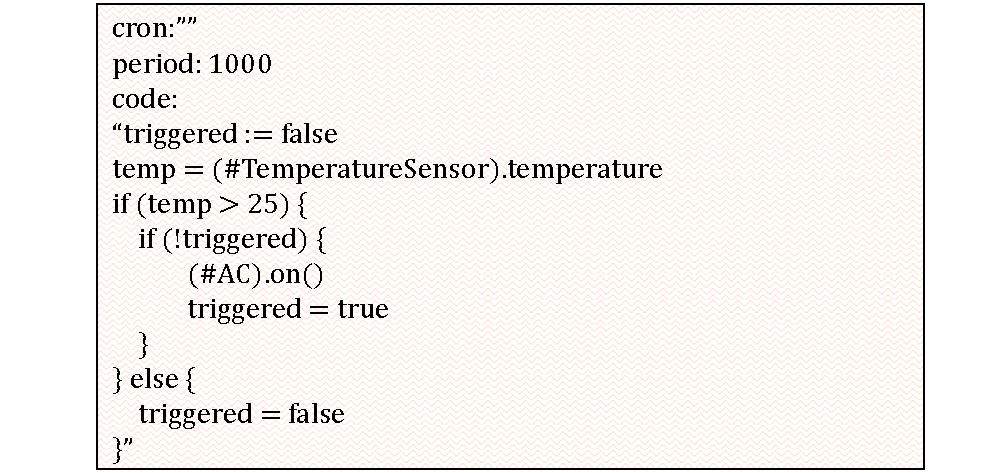
\includegraphics[width=\linewidth]{figs/figure1_b.pdf}\par
{\small (b) Triggered flag}\par\smallskip

\includegraphics[width=\linewidth]{figs/figure1_c.pdf}\par
{\small (c) level 유지 동안 재발화}\par\smallskip
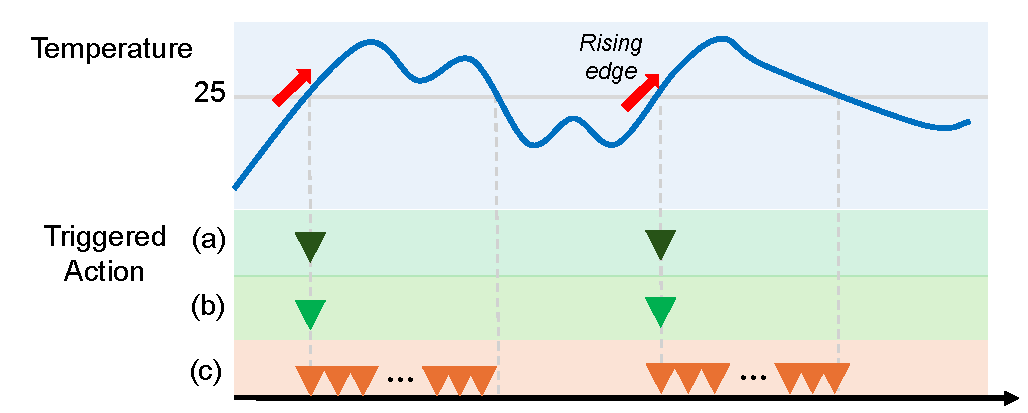
\includegraphics[width=\linewidth]{figs/figure1_trace.pdf}\par
{\small (d) Action traces}
\caption{한 의도(``온도가 25°C를 넘어설 때마다 에어컨을 켜줘'')의 세 가지 lowering 스케치와 action trace. (a)와 (b)는 동일한 trace를 만들고, (c)는 임계 초과 동안 매 tick 발화한다.}
\label{fig:idiom}
\end{figure}

\textbf{기존 검사가 부족한 이유.}
기존 IoT 자동화 검증 프레임워크는 사용자 의도가 아니라 고정된 사전 정의 기준을 겨냥한다. 많은 연구가 손으로 작성한 trigger-action rule을 검사한다. 예컨대 model checker는 safety 속성·rule 간 충돌·보안 정책을 증명하고(예: AutoTap~\cite{autotap}), 런타임 모니터는 채굴된 invariant로부터의 이탈을 flag한다~\cite{hawatcher}. 이 한계는 부주의가 아니라 설계 패러다임의 귀결이다. 사용자가 rule을 직접 작성할 때는 rule 자체가 ground-truth 의도이며, 검증할 가치가 있는 핵심 위험(rule 충돌, 보안 위반)은 특정 task의 고유한 의도 행동을 참조하지 않고도 정의할 수 있다. 그러나 사용자가 author에서 prompter로 옮겨가면 검증 패러다임이 근본적으로 바뀐다. LLM이 자연어 요청에서 코드를 합성하는 순간, 사용자의 원래 발화와 생성된 산출물은 조용히 어긋날 수 있는 별개의 분리된 실체가 된다. 이 생성 워크플로에서 intent-conformance가 결정적이면서도 다뤄지지 않은 검사 지점으로 떠오른다.

이 생성 환경에서 그 갭은 활짝 열려 있고, 갭을 잇는 일은 하나의 질문에 달려 있다: test oracle이 이미 존재하는가? 알고리즘성 IoT 코드용 생성기는 text-to-SQL이 관계형 denotation을 검증하듯 실행 가능한 테스트 스위트나 라벨된 정확도로 출력을 쉽게 검증할 수 있다. 이런 도메인에서 intent-conformance는 사실상 해결된 문제다(예: GPIoT~\cite{gpiot}). 그러나 reactive 자동화에는 그런 기성 oracle이 없다. 그래서 자연어→자동화 생성기들은 더 약한 proxy로 물러선다: 스키마 유효성(프레임워크가 JSON 구문을 받아들이는지), 기기 grounding feasibility, ground-truth 명령과의 어휘 매칭, 또는 LLM judge 평가. 생성된 rule을 사용자에게 되보여주는 프레임워크조차 그 실행 코드에 대한 검증이 아니라 수동의, 오류가 잦은 human-in-the-loop 확인에 의존한다(예: AwareAuto~\cite{awareauto}). 지금까지 어떤 시스템도 reactive-temporal 코드가 사용자의 행동 의도를 시간에 걸쳐 충실히 실행하는지를 결정론적으로 검증하지 않는다. 근본적으로 빠진 조각은 더 유능한 언어 모델이 아니라 검증 가능한 reference specification이다.

\textbf{왜 LLM judge로는 안 되는가.} 사용자 의도를 직접 겨냥하는 남은 대안은 다른 LLM에게 코드가 요청과 일치하는지 묻는 것이다. 그러나 LLM judge는 배포 게이트로 쓰기에 너무 불안정하다. 배포 결정은 이진이다: 행동이 동일한 두 프로그램은 같은 배포/기각 verdict를 받아야 한다. 그런데 우리는 idiom만 다른 행동 보존 프로그램에서 LLM judge의 verdict가 temperature 0에서조차 뒤집힘을 발견한다(\S3). 더 큰 모델도 뒤집히고, 클라우드 모델은 엣지의 프라이버시·지연 제약을 위반한다. verdict가 코드의 표면형을 따라가는 게이트는 배포를 막는 데 부적합하다.

\textbf{OVLA.} 이 난제들을 해결하기 위해 우리는 OVLA를 제안한다. 핵심 아이디어는 \emph{빠진 reference specification을 작성(authoring) 시점에 유도}하고, 이를 결정론적 검증 기준으로 활용하는 것이다. 먼저 OVLA는 자연어 요청에서 후보 Timeline IR을 만든다. 다음으로 시스템은 이 IR의 결정론적 평문 rendering을 생성해 사용자가 검토·확인하게 한다. 이렇게 확인된 IR이 자동화별 behavioral oracle이 된다. 생성된 JoI 코드는 IR이 정의하는 유한한 transition point 집합 위의 bounded trace-equivalence로 이 oracle에 대해 검증된다. 두 산출물을 그 지점들에서 합성된 이벤트(타이머 만료, 조건 임계, cycle 재시작 등) 위에서 실행하고 결과 action trace를 비교한다. LLM은 \emph{생성} — IR 제안과 코드로의 lowering — 에 국한되며, rendering 단계와 동치 검사는 모두 결정론적이고 LLM-free다. 덕분에 적합 판정된 자동화는 클라우드 측 검토 없이 엣지에서 안전하게 배포될 수 있다. lowering이 확률적 LLM에 의존하기 \emph{때문에 바로} 결정론적 검사기가 필요하다.

\textbf{Scope와 가정.}
OVLA는 명시적 reactive-temporal 행동을 지정하는 자연어 명령을 대상으로 한다. 모호하거나 감성적인 목표(``아늑하게 해줘'')에서 의도를 추론하는 것은 별도의 intent-elicitation 과제로, 직교하는 문헌(예: Sasha~\cite{sasha}, SAGE~\cite{sage})이 다루며 엄격히 scope 밖이다. 지정 가능한 명령 안의 잔여 모호성은 verifier가 아니라 OVLA의 결정론적 rendering 단계가 의도적으로 드러내고 사용자 확인에서 해소된다.
IR 확인은 프로그래밍 과제가 아니라 평문 판단으로 제시된다. reactive-temporal 자동화에서 사용자가 제어하는 차원은 제한적이고 열거 가능하며(시작 시각, period, trigger와 조건, action과 인자, sustain·delay duration), Timeline IR은 이 슬롯들만 표현하고, 결정론적 rendering은 이를 읽기 쉬운 타임라인으로 그대로 표시한다(\S8.1). 따라서 IR 승인은 명령이 지정한 유한 제어 슬롯에 대한 닫힌(closed) 판단이지 임의의 형식 속성 작성이 아니다.

\textbf{Two-layer 보장.} 우리는 검증 scope의 경계를 명시적으로 정의한다.
\textbf{Layer A (NL→IR)}에서 시스템은 의도를 IR로 포착해 평문으로 제시하지만, 비전문가의 확인 성공률 \emph{자체}는 이번에 human-subjects study로 측정하지 않는다(\S9). \textbf{Layer B (IR→code)}에서는 IR이 승인된 후, OVLA가 생성 코드가 그 표시된 IR로부터 유계 행동 영역 안에서 조용히 어긋나는 것을 막는다. OVLA의 기술적 보장은 확고히 Layer B에 있다.

\textbf{배포 환경.} 우리는 클라우드가 아닌 가정 엣지 기기를 가정한다 — 프라이버시(센서 데이터가 집을 떠나지 않음)와 지연 감소를 위해서다.
이 환경은 클라우드 LLM judge를 배제하므로 검증 게이트는 LLM-free 결정론 검사여야 한다. 결과적으로 하나의 설계 결정이 신뢰(비확률적 판정)와 배포 가능성(모델 호출 0의 ms 수준 로컬 실행)을 동시에 제공한다.

\medskip\noindent\textbf{Contributions.}
우리가 아는 한 OVLA는 LLM 생성 reactive-temporal IoT 자동화에서 intent-conformance를 결정론적 배포 전 검증 검사로 바꾼 최초의 시스템이다. 확률적 judge나 피상적 수동 검토 대신, 사용자가 확인한 behavioral IR을 권위 있는 test oracle로 세움으로써 이를 달성한다.
\begin{itemize}
\item \textbf{C1. Timeline IR:} 두 역할을 동시에 수행하는 통합 표현을 소개한다: (a) 사용자 검증을 위해 결정론적으로 평문 렌더링되는 표면, (b) reactive-temporal 코드 검증을 위한 기계 검사 가능 behavioral reference. 승인된 NL 문장은 (a)만, 형식 속성은 (b)만 할 수 있는 반면, 우리 기여는 둘 다 달성하는 단일 표현에 있다. 확인 가능한 temporal IR 생성은 선행 연구에도 있으므로, 우리의 차별적 주장은 결정론적 LLM-free 검증, 자동 rendering, 로컬 on-device 동작의 새로운 통합이다(\S2).
\item \textbf{C2. 결정론적 배포 게이트:} IR→FSM→boundary event→bounded trace-equivalence로 이어지는, LLM 개입 없이 전부 실행되는 end-to-end 파이프라인을 제안한다. 게이트는 fail-closed 정책으로 동작한다: 통과는 즉시 배포, 실패는 자동 수리 또는 기각. 게이트가 프로그램을 기각하면 정의된 observation model 아래 진짜 행동 발산이 보장된다(rejection-soundness).
\item \textbf{C3. On-device 실현:} 생성 단계는 fine-tuning 없는 최대 9B 파라미터의 4-bit 양자화 모델을 쓰고, 검증 게이트는 LLM 실행을 완전히 우회한다. 결과적으로 검증은 median 기준 약 1ms에 로컬로 완료된다. OVLA의 검증 보장은 생성 모델의 크기나 품질에 의존하지 않는다.
\item \textbf{C4. 평가:} rendering 충실성(\S8.1)과 verifier 검출 정확도(\S8.2)를 평가하고, silent IR→code 발산 9.2\%를 0으로 줄여 시스템 안전성을 실증하며(\S8.3), on-device 실행 오버헤드와 배포 가능성(\S8.4)을 컴포넌트별 분석으로 측정한다.
\end{itemize}

\textbf{기여의 초점.} OVLA는 사용자 승인을 통과하고도 살아남는 failure mode를 제거한다: 승인된 IR이 문제없어도, 이어지는 reactive-temporal lowering 단계가 미묘한 state·timer·boundary 오류를 끼워 넣어 배포 코드가 어긋나게 만들 수 있다. OVLA는 정확히 이 오류들을 가로채고 교정하도록 설계된 결정론적 on-device 게이트다.

\section{Related Work and Positioning}

홈 자동화의 검증은 처음부터 열린 문제가 아니었다. 사용자가 rule을 직접 작성하던 시절에는 rule 자체가 분석 대상 산출물이었고, 형식 기법이 그것을 고정 속성에 대조해 검사할 수 있었다. 실행 가능한 테스트가 딸린 도메인에서 코드가 생성될 때는 그 테스트가 oracle이었다. 두 환경 모두에서 검증이 시작되기 전에 검사 가능한 reference가 이미 존재했다. LLM이 이 워크플로에 들어온 건 실용적 이유에서다: 작성(authoring)이 병목이다 — 최종 사용자는 슬롯 기반 rule조차 작성·디버깅에 어려움을 겪고, 더 풍부한 reactive-temporal 행동은 그들이 아예 쓸 수 없는 코드를 요구한다. 이 전환은 사용자를 author에서 prompter로 바꾸고, 요청과 그것을 구현하는 산출물을 분리하며, 이전 검증이 기대던 바로 그 reference를 제거한다. 따라서 우리는 선행 연구를 각 시스템이 무엇을 reference로 검사하는가로 조직한다.

\textbf{검증 reference가 이미 존재하는 경우.} 손으로 작성한 TAP rule을 형식 기법으로 검증하는 연구가 풍부하다. AutoTap~\cite{autotap}은 TAP rule을 transition system으로 모델링해 사용자가 고른 LTL safety 속성 템플릿을 만족하도록 합성·수리한다. TAPInspector~\cite{tapinspector}는 타이밍 인지 rule 집합을 safety/liveness 위반에 대해 model-check하고 TAPFixer~\cite{tapfixer}는 그런 위반을 수리한다. 관련 분석들은 rule 간·보안 취약점을 밝혀내고~\cite{iruler,soteria}, HAWatcher~\cite{hawatcher}는 배포된 자동화를 채굴된 invariant에 대해 런타임 모니터링한다. 이 계열에서 결정론적 검증이 가능한 이유는 reference가 사전에 고정되어 있기 때문이다: safety 속성, 충돌 없음, 보안 정책. 사용자가 rule을 직접 작성하므로 rule 자체가 분석 대상이고, task별 의도 reference는 결코 필요하지 않다.

도메인이 실행 가능한 oracle을 제공하는 생성 대상도 마찬가지다. GPIoT~\cite{gpiot}는 on-device fine-tuned SLM으로 자연어 요구사항에서 신호처리·ML 알고리즘 코드를 생성하고 pass@k 실행 테스트로 결과를 검증한다. IoT 밖에서는 text-to-SQL이 생성 쿼리를 gold 쿼리의 denotation에 대조해 검증하고~\cite{spider}, CodeT~\cite{codet}와 Self-Debug~\cite{selfdebug}는 unit test로 생성 코드를 검증한다. \emph{두 계열 모두에서 검증을 가능하게 한 것은 이미 존재하던 검사 가능한 target이었다 — 고정 속성이든, 테스트 스위트든, gold denotation이든.}

\textbf{LLM 생성 reactive 자동화: 기성 reference 없음.} LLM 생성 reactive 자동화에는 그런 target이 없다: 의도된 행동은 사용자의 요청에만 이름 붙어 있고, 어떤 벤치마크나 테스트 스위트도 그 미래 action 시퀀스를 라벨하지 않는다. 빠진 reference는 TAP rule보다 대체하기도 더 어렵다. TAP rule도 trigger, stays-for duration, cron형 스케줄 같은 temporal 행동을 담지만, 거기서 그것은 플랫폼 \emph{primitive}다: 작성자가 슬롯을 채우면 엔진이 메커니즘을 구현하므로 슬롯 오류는 rule 표면에 보인다. JoI 스크립트 같은 reactive-temporal 코드에는 edge 탐지·지속 조건·카운팅을 위한 그런 primitive가 없다. 작성자 — 여기서는 LLM — 가 영속 변수·조건·per-tick 실행으로 메커니즘을 \emph{idiom}으로 구현해야 한다. 메커니즘 오류는 silent하고, 바로 거기가 lowering 버그가 생기는 곳이다.

이 체제의 일부 시스템은 LLM 출력을 결정론적으로 검사하지만, 여전히 고정 기준에 대해서다. AutoIoT~\cite{autoiot_maude}는 Maude rewriting logic으로 LLM 생성 rule을 4가지 rule 간 충돌 유형에 대해 검사한다. DS-IA~\cite{dsia}는 명령의 기기 grounding feasibility를 결정론적 cascade로 검사해 실행 전 infeasible 명령을 fail-closed로 기각한다. TaskSense~\cite{tasksense}는 sensing query를 실행 가능한 tool-calling DAG로 번역하고, LLM 기반 solvability 검사로 거른 뒤, plan의 의존성 그래프가 toolset grammar의 subgraph인지 결정론적으로 검사한다. 두 검사 모두 구조적 well-formedness를 확립할 뿐이고, 유일한 행동 reference인 손으로 작성한 ground-truth plan은 오프라인 평가에만 존재한다. AgentSpec~\cite{agentspec}은 결정론적 DSL로 LLM agent에 trigger-predicate safety rule을 런타임에 강제하지만, 그 rule은 처리 중인 요청에서 유도된 것이 아니라 고정된 수작성 rule이다. \emph{이 검사들 대부분은 결정론적이지만 reference는 여전히 사전 정의된 기준이다. 사용자가 실제로 요청한 행동은 여전히 한 번도 reference가 아니다.}

생성 시스템 자체는 더 약한 검사로 물러선다. ChatIoT~\cite{chatiot}는 여러 LLM agent로 자연어를 Home Assistant 자동화로 번역하고 별도의 ``Evaluator'' agent가 형식 준수와 요청 충족을 평가하게 한다. Giudici 등~\cite{giudici2025}은 프레임워크가 JSON을 파싱하면 생성 routine을 수락한다. IoTGPT~\cite{iotgpt}는 가상 SmartThings 환경에서 API 위반과 런타임 오류는 잡지만 의도 불일치는 못 잡는다. AwareAuto~\cite{awareauto}가 가장 멀리 간다: event/state 모드, delay, 분기, 시퀀싱을 갖춘 확인 가능한 reactive-temporal rule을 만들어 패널로 사용자에게 제시하고 실행 가능한 JSON으로 lowering한다. \emph{이 계열 전반에서 자동 검사는 형식 적합성, API 유효성, 기기 grounding feasibility에서 멈춘다. AwareAuto에서조차 의도 일치는 연구자 annotation으로 평가되고, 사용자에게 보이는 확인 텍스트는 결정론적 rendering이 아니라 생성된 산문이다. 결과적으로 이들 중 어느 시스템도 생성 코드가 사용자 의도대로 동작하는지 검증하지 않는다.}

생성 산출물이 사용자 의도와 일치하는지 직접 묻는 연구는 드물다. LACE~\cite{lace}는 생성된 접근제어 정책을 결정론적 템플릿으로 자연어로 역번역하고 fine-tuned NLI 모델로 원 요청과의 의미 동치를 판정한다. SimuHome~\cite{simuhome}은 시간 가속 시뮬레이터에서 agent 행동을 goal state에 대조해 판정하며, 18개 LLM agent가 자신의 reactive-temporal 오류를 대부분 자가 수정하지 못함을 보인다(\S3). 그러나 그 goal은 사용자가 확인한 것이 아니라 벤치마크가 작성한 것이고, 배포를 게이트하는 게 아니라 agent를 평가한다. \emph{의도를 직접 다루는 곳에서조차 의도의 ground truth는 사용자뿐이므로, model-only verdict는 자기 자신을 인증하는 셈이다 — LACE가 보고한 ``100\% correctness''처럼.}

두 시스템이 우리 문제의 각 축에서 OVLA에 가장 가깝다: reference 축의 LACE(생성 산출물을 사용자 요청에 대조 검사)와 artifact 축의 AwareAuto(확인 가능한 reactive-temporal 표현 구축). 그러나 LACE는 정적 정책 위에서 확률적으로 판정하고, AwareAuto는 lowering된 코드의 행동을 끝내 검증하지 않는다. OVLA는 정확히 둘이 멈춘 곳에서 시작하며, 사용자를 reference의 유일하게 정당한 원천으로 취급한다: 빠진 reference를 작성 시점에 유도하고, 사용자 확인 IR을 behavioral oracle로 삼아, 생성된 reactive-temporal 코드를 결정론적 LLM-free trace-equivalence로 — 배포 전에, 기기 위에서 — 검사한다. 생성과 검증을 결합하는 것 자체는 이 분야의 표준 관행이며 우리의 신규성 주장이 아니다. 신규성은 사용자 확인 behavioral reference, 결정론적 LLM-free 검사, on-device 동작의 결합에 있으며, 이 셋을 함께 제공하는 단일 선행 시스템은 없다.

\section{Problem and Motivation}

\S1과 \S2는 명확한 과제를 남긴다: LLM 생성 reactive-temporal 코드가 사용자 의도대로 동작하는지를 배포 전에 결정하는 게이트가 필요하다. 이 섹션은 먼저 우리 환경에서 그런 게이트가 충족해야 할 요구사항을 세우고, 다음으로 대안 후보 검사 접근들을 그에 대조하며, 마지막으로 남은 후보인 LLM judge를 직접 측정해 우리 해법의 동기를 만든다.

\textbf{배포 게이트의 세 요구사항.}
\begin{itemize}
\item \textbf{R1 (Reference).} 사전 reference가 없다. 의도된 행동은 오직 사용자의 방금 요청으로 결정되며, 검사 가능한 산출물로 제공되지 않는다. 알고리즘성 코드는 입출력 쌍이라는 실행 가능 oracle을 지니고 테스트 실행으로 검사된다(GPIoT~\cite{gpiot}, \S2). reactive-temporal 코드의 ``정답 출력''은 어떤 외부 소스도 라벨하지 않는 미래의 기기 action 시퀀스다. reference는 조회되는 것이 아니라 구성되어야 한다.
\item \textbf{R2 (Stability).} 배포 결정은 이진이다: 같은 행동의 두 프로그램은 같은 배포/기각 verdict를 받아야 한다. 행동 보존 rewrite 아래 verdict가 흔들리는 검사기는 개별 판정의 품질과 무관하게 게이트로 부적합하다.
\item \textbf{R3 (On-device).} 센서 데이터는 집을 떠나선 안 되고(프라이버시) verdict는 즉각적이어야 하므로(지연), 게이트는 클라우드 왕복 없이 엣지에서 실행되어야 한다.
\end{itemize}

\textbf{후보 1: 구문적·구조적 비교.} 가장 직관적인 검증 방법은 생성 코드를 reference 텍스트와 직접 매칭하는 것이다. 그러나 \S1의 온도 제어 예시(그림~\ref{fig:idiom})가 보이듯, 동일한 사용자 의도가 구문적으로 이질적인 idiom들(이전/현재 비교 vs.\ triggered flag)로 실현될 수 있는 반면, 버그 구현이 오히려 요청을 가장 닮았다. 실제로 실행 tick 하나, 비교 하나만 다른 near-miss 버그는 유효한 코드 변형과 똑같아 보일 수 있다. 구문적·구조적 매칭은 다양한 올바른 변형을 검증하지도, 미묘한 버그를 분리하지도 못하므로 soundness도 completeness도 충족하지 못한다. 동치는 구문이 아니라 실행 행동으로 판정되어야 한다.

\textbf{후보 2: 생성 모델의 자가 검사.} 코드를 만든 모델에게 검사·수리를 시킬 수 있다. SimuHome~\cite{simuhome}은 18개 모델로 이 방법을 평가했다: 자가 수정 회복률은 시간 기반 오류 8.0\%, 이벤트 기반 오류 18.5\%, 협조적 스케줄링 0.0\%였다. 특히 oracle을 제공해도 성공률은 67\% 이하에 머물렀다. 이 결과에 근거해 저자들은 agent가 자기 plan의 결함을 탐지하지 못한다고 결론지었다. 코드를 생성한 바로 그 확률적 프로세스에 맡기는 사후 자가 검사는 신뢰할 수 있는 품질 게이트가 될 수 없다.

\textbf{후보 3: 코드의 인간 검사.} 생성 코드를 사용자에게 보여주고 승인받을 수 있다. 그러나 TAP-Debug~\cite{tapdebug}의 선행 연구는 비전문가가 raw rule의 기본적인 IF(event)·WHILE(state) 조건조차 자주 오독함을 보였다: 구체적으로 50개 대조 조건 세션 중 21개에서 오독이 발생했고, 그 전부가 이어서 task에 실패했다. 단순한 두 슬롯 TAP rule에서도 이런 오류가 나는데, 영속 변수와 per-tick 실행으로 메커니즘을 구현하는 복잡한 reactive-temporal 코드를 사용자가 성공적으로 검사하리라 기대하는 것은 무리다. 사용자에게 보여줄 것은 raw 코드가 아니라 읽기 쉬운 표현이어야 한다 — 이것이 \S5의 결정론적 rendering의 동기이기도 하다.

\textbf{남은 후보: LLM judge.} 남은 것은 요청과 코드를 별도 LLM에 넘겨 둘이 일치하는지 확인시키는 것이다. 이 접근은 일견 그럴듯하고 실제로 쓰이며(ChatIoT의 Evaluator, \S2), 기존 문헌이 이를 기각하지 못한다. 그래서 우리는 OVLA의 IR·verifier와 무관하게 이 후보가 R2를 충족하는지 평가한다.

행동이 정확히 동일(trace-exact)하고 idiom만 다른 프로그램 쌍들을 제시하고 judge의 수락/기각 verdict가 얼마나 자주 뒤집히는지 측정했다. temperature 0의 결정론적 설정에서조차 9B 모델은 쌍의 27\%에서, 강한 클라우드 모델은 10.6\%에서 뒤집혔다. rewrite 유형은 표면 rewrite(SEL = selector 순서, AND = $A{\wedge}B{\leftrightarrow}B{\wedge}A$, VAR = 변수명 변경)와 논리/산술 rewrite(ADD = $x{+}n{\leftrightarrow}n{+}x$, BR = 분기 교환, DN = 이중 부정, DM = De Morgan, IDM = idiom 교체)로 나뉜다. 그림~\ref{fig:instability}이 보이듯, 순수 표면 rewrite만으로 9B judge verdict의 최대 9\%(클라우드 judge 14\%)가 뒤집혔고, 논리·산술 rewrite는 최대 81\%까지 뒤집었다. 이를 보이는 데 ground-truth 라벨은 필요 없다 — 뒤집힘 자체가 불안정성의 증거다.

핵심은 miss rate가 아니다. 깨끗하게 주입된 버그에서 강한 모델은 실제로 유능한 탐지기다. 요점은 \emph{어떤} 확률적 judge든 행동 보존 rewrite 아래 불안정한 배포 정책을 낳는다는 것이다. 이 불안정성은 더 큰 모델에서도 지속되고, 다수결 투표도 temperature-0 기준선 아래로 줄이지 못한다 — 투표는 샘플링 노이즈는 완화하지만 표면형에 대한 체계적 의존은 상쇄할 수 없기 때문이다(표~\ref{tab:instab}). 이는 R2를 위반하며 마지막 후보를 탈락시킨다. 대조적으로 OVLA의 verdict는 유계 trace 집합 위의 행동에만 의존하므로 같은 rewrite 아래 flip rate가 구성상 0이다.

\begin{figure}[t]
\centering
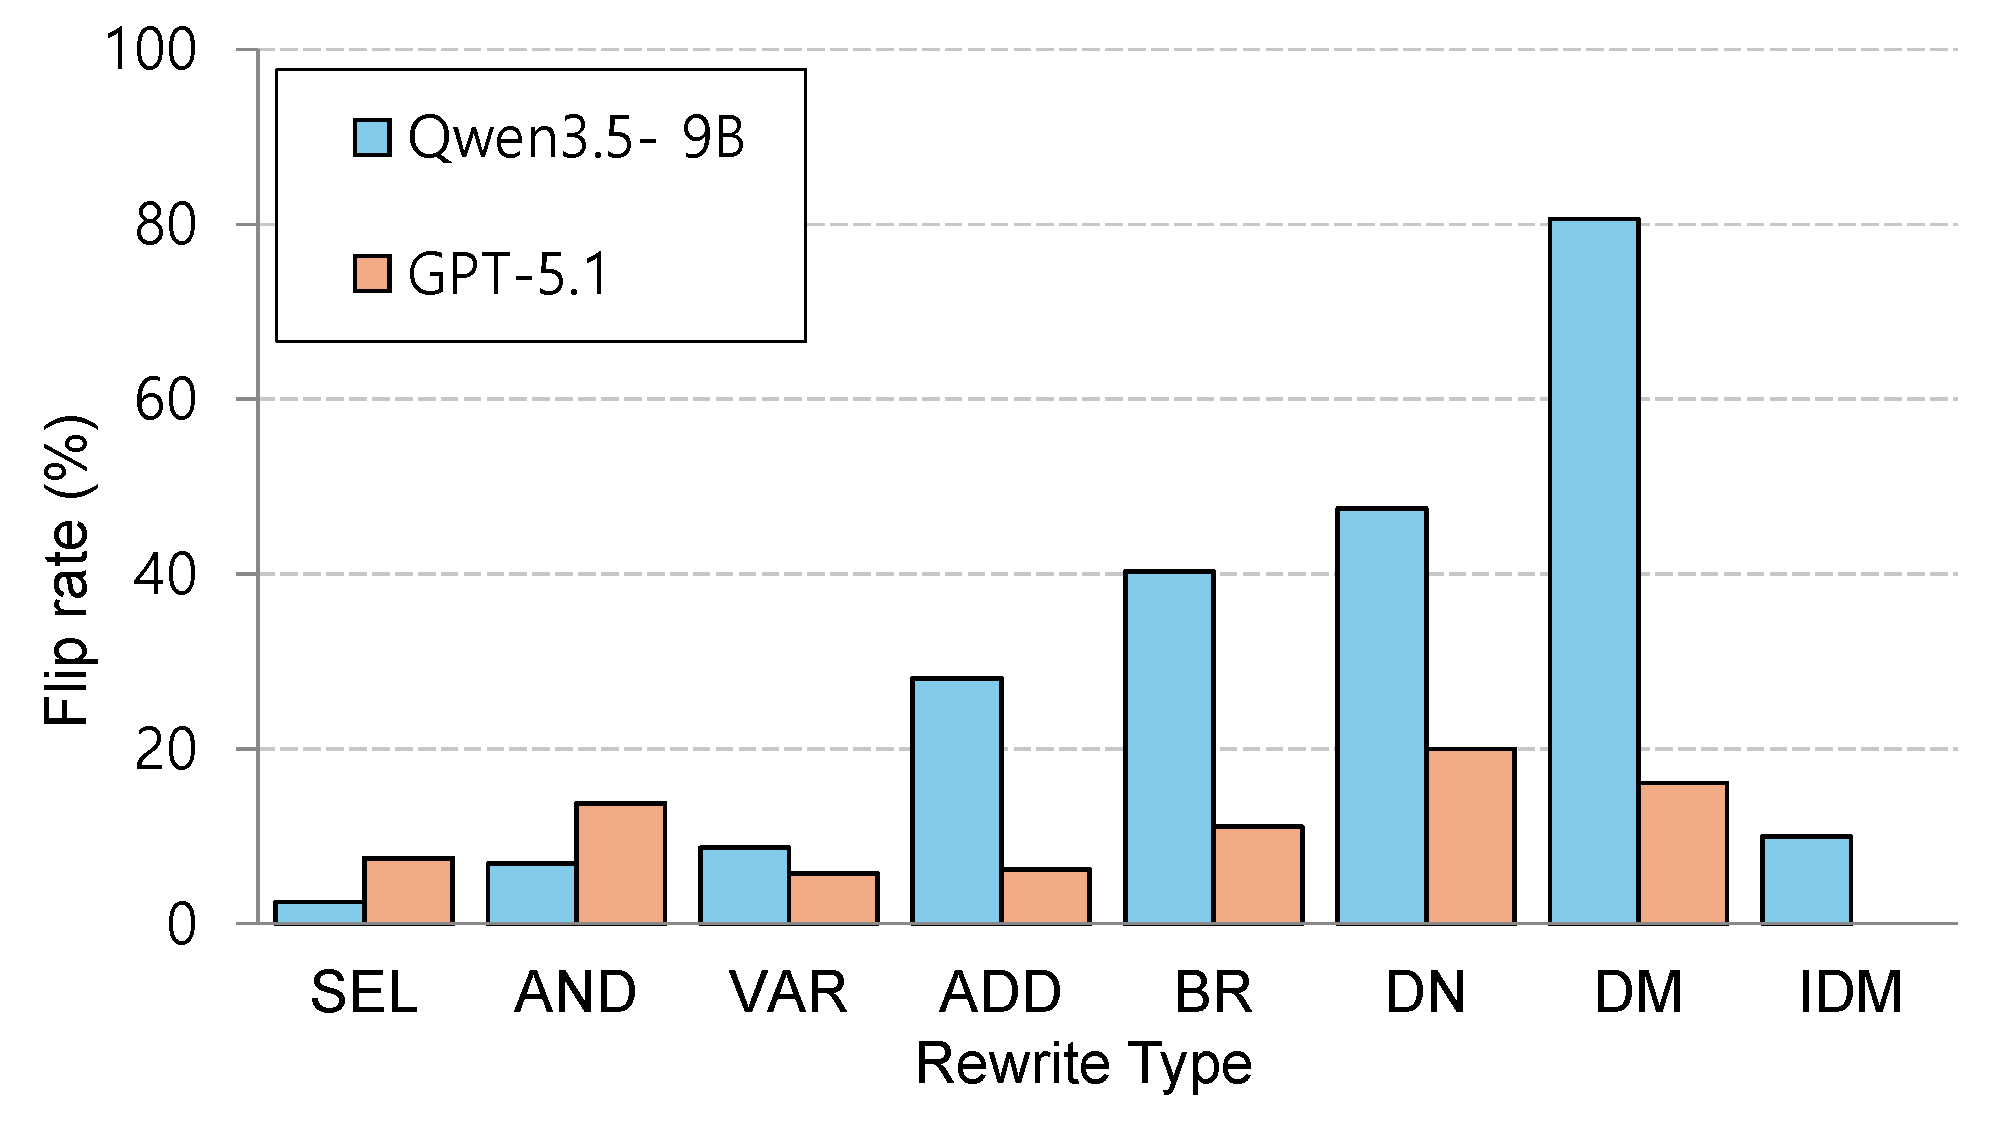
\includegraphics[width=\linewidth]{figs/instability.pdf}
\caption{행동 동일 프로그램에 대한 rewrite 유형별 LLM judge verdict flip rate (temperature 0).}
\label{fig:instability}
\end{figure}

\begin{table}[t]
\centering
\caption{judge 구성별 전체 flip rate; OVLA의 trace 검사는 같은 rewrite에서 하나도 뒤집히지 않는다.}
\label{tab:instab}
\begin{tabular}{lcc}
\toprule
Judge configuration & 9B & GPT-5.1 \\
\midrule
deterministic (temp=0) & 27.0\% & 10.6\% \\
+ sampling (temp=0.7) & 34.4\% & 12.8\% \\
+ majority vote (K=5) & 31.2\% & 13.5\% \\
\textbf{OVLA (deterministic trace)} & \textbf{0\%} & \textbf{0\%} \\
\bottomrule
\end{tabular}
\end{table}

\textbf{살아남는 설계.} 모든 후보가 탈락한 지금, 요구사항을 다시 읽으면 답의 윤곽이 드러난다. R1에 의해 reference는 사용자가 확인한 의도에서 \emph{유도}되어야 하고, R2에 의해 검사는 구문이 아닌 행동(trace) 위에서 결정론적이어야 하며, R3에 의해 LLM 호출 없이 엣지에서 가벼워야 한다. 셋을 동시에 만족하는 산출물이 Timeline IR(\S5)이고, 그 위의 결정론적 trace-equivalence 검사가 verifier(\S6)다. 이 동기 실험의 judge는 NL을 코드와 비교한다.

\begin{figure*}[t]
\centering

\includegraphics[width=\textwidth]{figs/system.pdf}
\caption{OVLA 시스템 개요. ①{--}⑤ 생성, ⑥{--}⑦ 검증; 점선 화살표는 counterexample 유도 수리 루프다.}
\label{fig:arch}
\end{figure*}

\section{System Overview}

OVLA는 \S3의 설계를 2-phase 파이프라인으로 구현한다. authoring phase에서 시스템은 사용자 명령에서 Timeline IR을 유도하고, 확인을 위해 그 IR을 렌더링하며, 확인된 IR을 실행 코드로 lowering한다. verification phase에서 시스템은 배포 전에 생성 코드를 확인된 IR에 대조해 검사한다. 핵심 경계는 파이프라인 전체에서 고정된다: LLM은 후보 산출물을 제안할 수 있지만, 배포에 영향을 줄 수 있는 모든 산출물은 결정론적 코드가 검사한다.

\textbf{실행 타깃.} 우리는 실행 DSL이 JoI인 상용 IoT 플랫폼의 엣지 허브 위에 OVLA를 인스턴스화한다. JoI 자동화는 시작 스케줄(\texttt{cron}), 재실행 간격(\texttt{period}), 스크립트 본문(\texttt{code})으로 구성된다. \texttt{period}가 양수면 본문이 매 tick 실행되며, edge 탐지·지속 조건·카운팅 같은 temporal 행동은 영속 변수와 일반 조건문으로 구현되어야 한다. 따라서 JoI는 lowering이 만들어내는 실행 산출물이자 verifier가 검사하는 산출물이다.

그림~\ref{fig:arch}은 전체 파이프라인을 보여준다. 첫 phase는 authoring이다: LLM 기반 생성 단계를 포함하지만, 사용자가 reference를 승인하기 전의 결정론적 게이트들도 포함한다. 둘째 phase는 verification이다: 승인된 IR과 생성된 JoI 코드를 입력으로 받아 LLM 호출 없이 실행된다.

\textbf{Phase 1: Authoring (결정론 게이트를 동반한 LLM 생성).} ① OVLA는 먼저 사용자의 자연어 명령을 분석한다. 이 분석은 자동화가 표현해야 할 temporal·행동 슬롯들 — 시작 시각, 반복 period, trigger 또는 조건, delay·sustain duration, 대상 action — 을 식별한다. 또한 명령을 연결된 기기 목록에 매핑하여, 자동화가 실행 가능하려면 어떤 기기와 그 기기들이 노출해야 할 service를 선택한다. ② 이어서 OVLA는 이 분석에서 후보 \textbf{Timeline IR}을 추출한다. ``후보''라는 말이 중요하다: 사용자 확인 전의 IR은 명령에 대한 시스템의 제안된 해석일 뿐이다. 어떤 코드도 생성되기 전에, 결정론적 \textbf{feasibility gate}(\S5)가 이 IR이 지원되는 구조 규칙을 따르는지 검사한다. 중첩 cycle이나 잘못 놓인 분기처럼 대상 실행 모델이 실현할 수 없는 구조를 기각한다. ③ IR이 이 게이트를 통과하면 OVLA는 그림~\ref{fig:arch}의 결정론적 \textbf{Rendered IR}로 렌더링한다. Rendered IR은 IR의 평문 뷰이지 새 자연어 명령이 아니다. ④ 사용자가 이 Rendered IR을 검토한다. 사용자가 확인하는 순간 Timeline IR은 그 자동화의 reference specification으로 고정된다. ⑤ 이 reference가 고정된 후에야 OVLA는 IR을 JoI 코드로 lowering한다.

\textbf{Phase 2: Verification (결정론, LLM-free).} ⑥ verifier는 두 산출물을 받는다: 확인된 Timeline IR과 생성된 JoI 코드. 확인된 IR이 behavioral reference다. verifier는 먼저 JoI 코드에 정적 syntax 검사를 수행한다. 행동 검사는 그림~\ref{fig:arch}의 아래 절반을 따른다. 확인된 IR로부터 OVLA는 enabled obligation들과 그 도달 가능 상태를 명시화하는 FSM을 유도한다. \textbf{Event Synthesis} 단계가 이 FSM에서 boundary 이벤트를 생성한다(\S6). 같은 합성 이벤트 집합이 두 결정론적 시뮬레이터에 공급된다: 확인된 IR을 실행하는 \textbf{IR-Sim}과 생성된 JoI 코드를 실행하는 \textbf{JoI-Sim}. 둘의 action trace가 \textbf{Trace-Equivalence} 단계로 전달되어 \S6의 observation model 아래 코드가 승인된 IR과 일치하는지 판정한다. ⑦ 통과한 프로그램은 배포된다. 실패한 프로그램은 곧바로 배포되지 않는다. 대신 verifier가 \textbf{counterexample}을 lowering 단계로 돌려보내고 JoI 코드만 재생성된다. 수리 중에 확인된 IR은 바뀌지 않는다 — 사용자가 승인한 reference로 남는다. 수리가 소진되면 OVLA는 자동화를 fail-closed로 기각한다.

\textbf{세 검사, 세 위치.} OVLA는 서로 다른 산출물에 각각 작동하는 세 가지 결정론적 검사를 쓴다. \textbf{feasibility gate}는 IR 추출 직후·lowering 전에 typed tree로서의 \emph{IR} 구조를 검사한다(\S5). \textbf{정적 syntax 검사}는 lowering 후·시뮬레이션 전에 \emph{생성된 JoI 코드}를 검사한다. \textbf{행동 trace-equivalence 검사}는 확인된 IR과 생성된 JoI 코드의 행동을 비교한다(\S6). 이 검사들은 서로 대체 불가능하다. 행동 검사가 핵심 배포 게이트이고, feasibility와 syntax 검사는 malformed 산출물이 그 게이트에 도달하는 것을 막는다.

\textbf{IR의 역할들.} 하나의 Timeline IR이 OVLA에서 네 역할을 수행한다. 첫째, 결정론적 rendering을 통해 사용자에게 노출되는 산출물이다. 둘째, 확인 후에는 verifier가 쓰는 behavioral reference다. 셋째, 시스템이 JoI 코드를 lowering하는 scaffold다. 넷째, 그 구조 클래스가 lowering example 라우팅에 쓰인다(\S7). OVLA는 의미 분석과 기기/service 매핑을 상류 단계로 사용하지만, 이 논문의 기여는 확인된 IR이 어떻게 렌더링되고, reference로 고정되고, lowering되고, 검증되는가에서 시작한다.

\begin{figure*}[t]
\centering
\begin{minipage}[t]{0.42\textwidth}
\centering
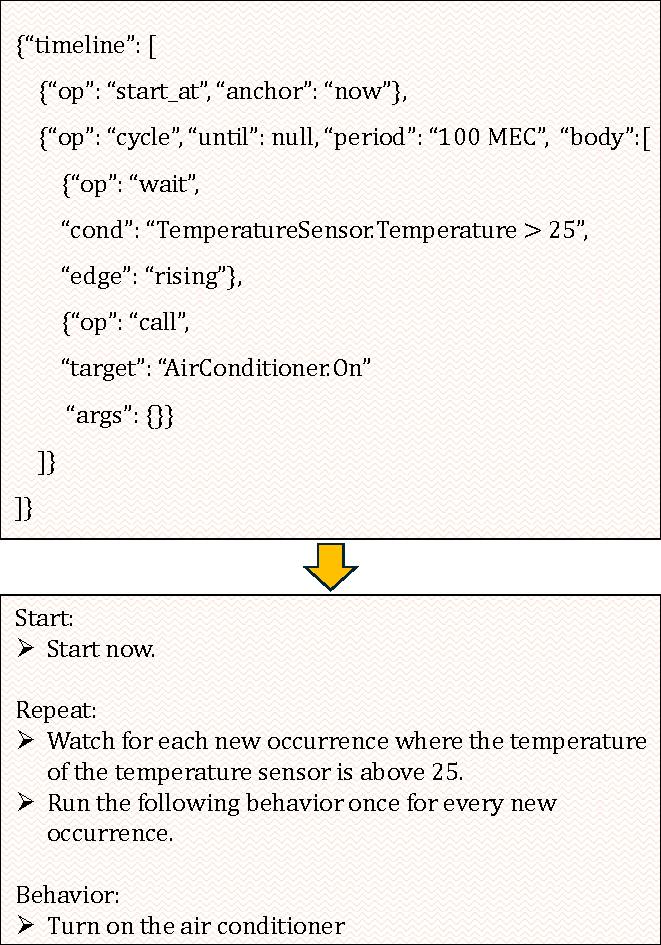
\includegraphics[width=\linewidth]{figs/Rendering1.pdf}\par
\small (a) 반복 edge trigger
\end{minipage}\hspace{0.04\textwidth}%
\begin{minipage}[t]{0.42\textwidth}
\centering
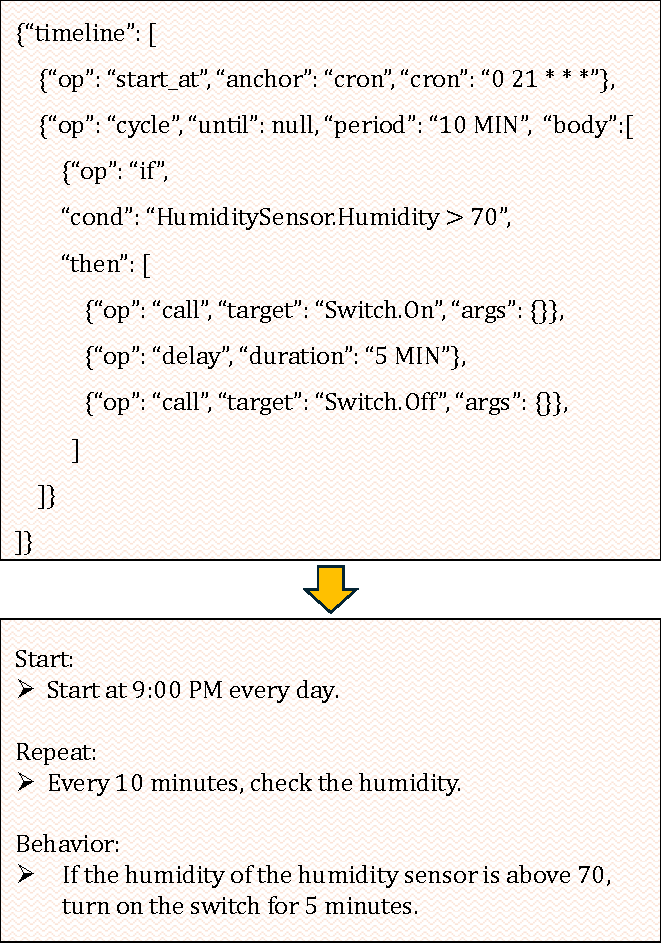
\includegraphics[width=\linewidth]{figs/Rendering2.pdf}\par
\small (b) 분기와 delay를 가진 스케줄 주기 검사
\end{minipage}
\caption{두 Timeline IR과 그 결정론적 평문 rendering.}
\label{fig:ir}
\end{figure*}

\section{Timeline IR}

Timeline IR은 사용자 확인과 결정론적 검증을 잇는 산출물이다. 두 역할이 있다. 첫째, 승인을 위해 사용자에게 보여주는 결정론적 rendering의 원천이다. 둘째, 승인되고 나면 verifier가 쓰는 기계 검사 가능 behavioral reference다. NL→IR은 LLM 단계지만 IR→rendering은 아니다. 결정론적 변환이므로 사용자에게 보이는 텍스트는 나중에 검사될 IR의 충실한 뷰다. rendering은 IR에 없는 행동을 만들어낼 수 없고, IR이 담은 행동을 숨길 수도 없다. 이런 의미에서, 표시되는 것이 곧 검사되는 것이다.

\textbf{닫힌 제어 차원과 primitive op.} 이 두 역할이 가능한 이유는 reactive-temporal 자동화의 제어 차원이 제한적이고 열거 가능하기 때문이다. 사용자 명령은 자동화가 언제 시작하는지(\texttt{start\_at}), 얼마나 자주 반복하는지(\texttt{cycle.period}), 어떤 trigger·조건을 기다리는지(\texttt{wait}의 condition·edge, \texttt{if}의 condition), 어떤 action을 어떤 인자로 수행하는지(\texttt{call}), 얼마나 기다리거나 지연하는지(\texttt{wait.for}, \texttt{delay}), 반복 행동을 어떻게 세고 멈추는지(\texttt{cycle.count}, \texttt{break})를 지정할 수 있다. Timeline IR은 이 차원들에 primitive operation을 할당하고 명명된 슬롯들을 타임라인 위에 직접 배치한다.

이 표현은 의도적으로 작다. 사용자에게 임의의 코드를 승인하거나 형식 속성을 작성하라고 요구하지 않는다. 대신 결정론적 rendering이, 행동이 전개되는 순서대로, 명령이 지정한 유한 제어 슬롯들을 노출한다. 따라서 사용자 승인은 그 슬롯들에 대한 닫힌 판단이다: 표시된 시작 시각, period, trigger, 조건, action, duration, 반복 행동이 의도한 자동화와 일치하는가. 같은 슬롯들을 verifier도 소비한다. 그러므로 IR은 rendering을 통한 승인 표면이자 생성 코드 검사를 위한 behavioral reference다. 아래의 구조 문법 G는 정확히 이 닫힌 operation 집합 위에서 정의된다.

\textbf{유한상태 관점.} Timeline IR은 자동화를 타임라인 위 유한한 obligation 집합으로 취급한다. obligation은 예정된 검사, 조건이 참이 되어야 하는 wait, guard가 경로를 고르는 분기, 발행되어야 하는 call, 다음 period에 반복되어야 하는 cycle 본문일 수 있다. IR은 recursion도 unbounded loop도 허용하지 않는다. 유계 timer·counter·분기·cycle만 쓰므로 verifier는 검사 horizon 안에서 관련 obligation들을 열거할 수 있다. Timeline IR은 완전한 timed-automaton model-checking 언어를 지향하지 않는다. 검사할 행동을 유한하고 명시적으로 만드는 운영적(operational) 관점이다.

\textbf{Typed tree와 구조 문법 G.} 구조적으로 IR은 typed tree다. 구조 문법 G가 어떤 부모-자식 관계와 제어 구조가 합법인지 지정한다. 예컨대 IR에는 정확히 하나의 \texttt{start\_at}과 최대 하나의 top-level cron 스케줄이 있다. \texttt{cycle}은 다른 \texttt{cycle.body} 안에 나타날 수 없다. \texttt{then}/\texttt{else} 블록은 \texttt{if}의 자식으로만 나타날 수 있다. \texttt{break}는 \texttt{cycle} 안에서만 합법이다. \texttt{cycle}은 period가 필수다 — \texttt{until} 조건은 선택이며, 없으면 cycle은 verifier의 유계 검사 horizon 안에서 반복한다(\S6).

IR이 이 구조 규칙들을 만족하는지는 결정론적으로 판정 가능하다. typed tree에 대한 같은 패스가 IR의 구조 클래스도 결정하는데, 가장 거친 수준에서는 IR이 top-level \texttt{cycle}을 포함하는지 여부다. OVLA는 이 클래스를 나중에 lowering example 라우팅에 쓴다(\S7). 구조 클래스는 생성을 돕지만 verifier의 수락/기각 결정에는 영향을 주지 않는다.

\textbf{Feasibility gate.} \S4의 feasibility gate는 추출된 IR의 구조 유효성을 G에 대조해 검사한다. IR 추출 직후·lowering 전에 실행된다. 추출된 IR이 중첩 cycle, 두 번째 top-level cron, 잘못 놓인 \texttt{then}/\texttt{else}, cycle 밖의 \texttt{break}를 포함하면, 게이트는 어떤 JoI 코드도 생성되기 전에 기각한다. 이 결정은 실증 결과가 아니라 구조적 결정이다: 게이트는 IR을 G의 규칙에 대조해 구성상(by construction) 검사한다.

이 게이트는 IR이 사용자의 진짜 의도를 포착했음을 증명하지 않는다. IR이 OVLA의 실행·검증 파이프라인이 구조적으로 지원하는 형태임을 확립할 뿐이다. LLM 추출기가 지원되지 않는 요청을 조용히 다른 합법 IR로 바꿔버리면, feasibility gate는 잘못된 의미의 합법 IR을 수락하게 된다. 그 잔여 의미 불일치는 의도적으로 rendering을 통한 사용자 확인에 맡겨진다. 이 때문에 추출기는 요청된 구조를 조용히 수리·단순화하지 않고 그대로 전사(transcribe)하도록 설계되었다.

primitive operator는 \texttt{start\_at}, \texttt{wait}(condition, edge, sustain duration), \texttt{delay}, \texttt{read}, \texttt{call}, \texttt{if}(then/else), \texttt{cycle}(period, count, until, body), \texttt{break}다. 그림~\ref{fig:ir}는 두 Timeline IR 예시와 그 결정론적 rendering으로 이 설계를 보여준다. 각 예시는 IR 내부 슬롯이 어떻게 사용자 대면 승인 텍스트가 되는지 보여준다.

그림~\ref{fig:ir}(a)는 \S1의 온도 예시를 다시 본다. ``온도가 25°C를 넘어설 때마다''라는 구절은 condition이 \texttt{Temperature > 25}이고 edge가 rising인 \texttt{wait}이 되어 \texttt{cycle} 안에 놓인다. rendering은 그 edge 슬롯을 ``each new occurrence''로, \texttt{call}을 ``Turn on the air conditioner.''로 노출한다. 그림~\ref{fig:ir}(b)는 스케줄 구동 자동화다. \texttt{start\_at} cron은 ``Start at 9:00 PM every day,''로, \texttt{cycle.period} 슬롯은 ``Every 10 minutes,''로 렌더링되고, \texttt{if}-\texttt{call}-\texttt{delay}-\texttt{call} 시퀀스는 하나의 조건부 행동으로 렌더링된다. 비어 있는 \texttt{else} 분기조차 ``Otherwise, do nothing.''으로 렌더링된다. 이것은 의도된 것이다: rendering은 행동 관련 슬롯을 빠뜨리지도 더하지도 않는다. 이 충실성 성질은 \S8.1에서 행동이 다른 IR 쌍 1,504개 전수에 대해 검증한다.

\section{Verifier}

\subsection{Observation Model: Transition-Boundary Conformance}

게이트는 단 하나의 질문을 판정한다: 생성된 JoI 코드가 승인된 IR과 \emph{동일한 행동을 보이는가}? \S2에서 관찰했듯 실행 DSL에는 IR의 제어 차원에 대응하는 primitive가 없으므로, LLM은 각 IR 행동을 idiom으로 구현한다: ``N분간 지속되면''은 매 폴링 tick마다 증가하다 임계에서 발화하는 counter가 되고, ``~할 때마다(edge)''는 발화 시 set되고 조건이 풀리면 reset되는 triggered flag(또는 이전/현재 비교)가 되며, ``N분마다''는 본문의 주기적 재실행이 된다. 따라서 하나의 IR 행동이 여러 유효한 idiom으로도, tick 하나·비교 하나가 어긋난 무수한 near-miss로도 나타나며(그림~\ref{fig:idiom}), 바로 이 idiom 구현 지점이 버그가 들어오는 곳이다. 그러므로 동치는 구문이 아니라 행동(trace) 위에서 판정되어야 한다.

OVLA는 가능한 모든 environment trace에 대한 동치 증명을 시도하지 않는다. 대신 reactive-temporal 행동이 변할 수 있는 지점들을 검사한다. 이 transition point에는 guard 임계, 조건 edge, delay·period 같은 time landmark, 그리고 internal state transition이 포함된다. internal state transition은 프로그램 자신의 영속 상태 변화다 — triggered flag가 set/reset되는 것, sustain counter가 발화 임계에 도달하는 것, cycle counter가 break를 일으키는 값에 도달하는 것. 이것들이 포함되어야 하는 이유는, 같은 센서 값이라도 내부 상태에 따라 다른 행동으로 이어질 수 있기 때문이다: 예컨대 그림~\ref{fig:idiom}(b)의 flag 기반 구현은 flag가 set되기 전에는 발화하고 그 후에는 침묵할 수 있다.

검사 공간이 유한한 이유는 둘이다. 첫째, Timeline IR은 유계 제어만 허용한다: recursion도 unbounded loop도 없으므로 한 실행 안에서 도달 가능한 내부 상태가 유한하다. 둘째, verifier는 유계 time horizon을 쓴다. 우리 구현에서 verifier는 1주를 시뮬레이션하며, 이는 모든 시각(time-of-day)·요일(day-of-week) 스케줄의 완전한 한 주기를 담는다. day-of-month나 month 같은 calendar 필드는 더 긴 시뮬레이션을 요구하지 않는다. 그 필드는 주간 패턴이 어느 날짜에 활성인지만 고르며, 활성 창 내부의 행동을 바꾸지 않는다. 따라서 verifier는 IR과 JoI 코드가 같은 calendar 날짜를 지정하는지 정적으로 검사한 뒤, 이미 시뮬레이션한 주간 행동을 재사용한다.

우리는 이 observation model을 \textbf{transition-boundary conformance}라 부른다. 이 model 아래 두 프로그램은, 고정된 유계 horizon에 걸쳐, 행동이 변할 수 있는 경계 — 임계 교차, 조건 edge, 타이머 만료, 다음 cycle 재시작 — 에서 action trace가 verifier의 tolerance 안에서 일치하면 conform한다. 이는 경계 집중 동치 판단이지 입력 공간 전체에 대한 증명이 아니다. 이 제한은 의도적이다. 이 제한이 검사를 결정론적·solver-free로 만들고 엣지 허브에서 돌 만큼 작게 만든다. 따라서 verifier는 heavyweight 형식 검증의 대체물이 아니라 배포 시점 필터로 읽어야 한다.

\subsection{Boundary Event Synthesis}

이벤트 합성기는 결정론적이고 LLM-free다. 승인된 IR에서 출발해, 실행의 각 지점에서 어떤 IR operation이 활성인지 기록하는 FSM을 유도한다. 각 primitive operation이 obligation을 기여한다: \texttt{call}은 action obligation을, \texttt{wait}·\texttt{delay}는 temporal obligation을, \texttt{read}는 값 관측 지점을, \texttt{if}는 guard 분기를, \texttt{cycle}·\texttt{break}는 반복·종료 구조를 기여한다. operation 간 순서가 차례를 부과하고, 분기가 guard를 더하며, cycle은 다음 period에 본문을 반복할 obligation을 더한다.

합성기의 목표는 observation model이 식별한 경계들에 대한 구체적 이벤트를 만드는 것이다. \texttt{wait(Temperature > 25, edge: rising)} 같은 rising-edge 조건의 경계는 온도가 25°C 이하에서 초과로 변하는 순간이다. \texttt{delay}의 경계는 delay가 만료되는 시각이다. \texttt{cycle}의 경계는 다음 period의 시작이다.

이 boundary 이벤트는 임의로 배치할 수 없다. 같은 온도 교차라도 자동화가 이미 \texttt{wait(Temperature > 25, edge: rising)} operation에 도달해 있어야 의미가 있다. 앞선 wait·delay가 끝나기 전, 선택되지 않은 분기 위, 도달하지 않은 cycle 반복에서는 쓸모가 없다.

따라서 합성기는 자동화가 실행의 어디에 있는지 알아야 한다. 어떤 wait·delay가 완료됐는지, 어떤 분기가 선택됐는지, 어떤 cycle 반복이 활성인지, 어떤 IR operation이 현재 enabled인지. FSM이 이 실행 상태를 명시적으로 기록한다.

이 FSM 상태를 써서 합성기는 각 대표 이벤트를, 해당 IR operation이 활성이고 trace를 바꿀 수 있는 시점에 배치한다. cell 안에서는 교차한 정확한 값이 중요한 게 아니라 이벤트의 타이밍과 도달 가능성이 중요하다. 불일치가 발견되면 verifier는 그 경계와 연결된 obligation으로 귀속시키고, 그 귀속이 \S4의 수리 루프로 돌아가는 counterexample이 된다.

합성은 JoI 표면 구문이 아니라 IR 의미론에 기반한다. read→센서 흐름을 추적하고 각 관련 값 도메인의 양 끝을 시딩해 scale·offset 실수가 드러나게 하며, 같은 센서를 두 번 읽어 비교하는 식에 대해서는 두 read 값의 관계를 같음·상승·하강 세 방향으로 시딩해 부호·방향 오류가 드러나게 한다. \texttt{abs}, \texttt{min}, \texttt{max} 같은 일부 IR 산술 헬퍼는 JoI에 직접 대응물이 없다. 그래서 lowering이 이를 조건부 코드로 펼치는데, 합성기는 그 펼침의 내부 경계들도 시딩한다. 이로써 예컨대 뒤집힌 clamp가 일반 임계값만 테스트됐다는 이유로 통과하는 것을 막는다. 합성기는 second-edge 시나리오 — 조건이 풀렸다가 나중에 다시 참이 되는 경우 — 도 포함하는데, 조건 해제 후 trigger가 다시 발화할 수 있는지 테스트하는 데 필요하기 때문이다. read-modify-write 누산기는 이 표적 boundary 시딩에서 제외되며 검사의 잔여 한계로 취급된다. 최종 합성 이벤트 집합은 IR 시뮬레이터와 JoI 시뮬레이터 모두에 그대로 공급되므로, 두 산출물은 동일한 입력 위에서 비교된다.

\subsection{Trace-Equivalence and Omission Detection}

두 시뮬레이터가 같은 합성 이벤트 위에서 실행되어 action trace를 만든다. verifier는 tick 양자화와 lowering의 폴링 period 선택을 흡수하는 timing tolerance 안에서 action들을 그룹화·중복 제거한 뒤 순서대로 비교한다. 이는 action 순서·다중성·경계 타이밍의 행동 관련 차이를 보존하면서, 무해한 폴링 수준 타이밍 변동만으로 verdict가 바뀌는 것을 피한다.

이 trace 비교는 commission과 omission을 모두 탐지한다. commission 오류는 JoI 코드가 IR이 허용하지 않는 action을 수행하는 것이다. omission 오류는 IR이 요구하는 action을 JoI 코드가 만들지 못하는 것이다. 핵심은 침묵이 trace의 일부라는 점이다. IR trace에 빈 구간이 있으면, 그 구간은 ``여기서는 아무 action도 일어나선 안 된다''고 말하는 oracle이다.

이것이 OVLA가 JoI trace를 승인된 IR을 시뮬레이션해 만든 기대 action trace와 비교하는 이유다. IR 시뮬레이터는 일어나야 할 action만 만드는 게 아니다 — 어떤 시간 구간에 action을 만들지 않음으로써 그 구간이 침묵해야 함도 지정한다. 예컨대 승인된 IR이 ``문이 열리면 5분 후 조명을 켠다''면, IR trace는 5분 delay 동안 아무 action이 없다가 delay 끝에 \texttt{Light.On()}을 담는다. 즉시 조명을 켜는 코드는 같은 최종 기기 상태에 도달할 수 있지만, 그 JoI trace는 IR trace가 침묵하는 구간 안에 action을 담는다. trace-equivalence가 이 타이밍 불일치를 탐지한다.

\subsection{What the Verdict Guarantees}

verdict는 결정론적이고 LLM-free다. \textbf{T1 (determinism)}: 같은 승인 IR과 생성 JoI 코드는 항상 같은 verifier verdict를 낳는다. \textbf{T2 (semantic rejection-soundness)}: verifier가 시뮬레이션 가능한 프로그램을 trace 불일치로 기각하면, 위에서 정의한 observation model 아래 실제 불일치를 찾은 것이다. parser나 simulator subset 밖의 프로그램은 fail-closed로 기각되며 semantic counterexample이 아니라 subset failure로 보고된다.

우리는 ``통과 ⇒ 정답''을 주장하지 않는다. 통과는 생성 코드가 유계 horizon과 tolerance 안에서 합성된 boundary trace 위에서 승인 IR과 일치했다는 뜻일 뿐이다. trusted computing base는 결정론적 verifier 자체다: IR 시뮬레이터, JoI 시뮬레이터, tolerance 정책, trace-equivalence 관계. 따라서 verdict는 코드를 생성한 LLM에 대한 신뢰에 의존하지 않는다. semantic 기각의 soundness는 모든 환경에 대한 증명이 아니라 시뮬레이터 충실성으로 환원된다. 우리는 검사를 두 방식으로 실증 평가한다: \S8.2는 construct 유도 mutation 테스트와, IR-FSM obligation·생성 JoI branch 양측에서 측정한 coverage로 verifier 검출과 합성 trace의 적정성을 스트레스 테스트하고, \S8.2는 게이트를 생성 자동화에 적용한 배포 결과를 측정한다. 생존 mutant들은 개별적으로 분석한다.

\subsection{Limits of the Check}

한계는 observation model에서 직접 따라 나온다. 1주 horizon은 정적 calendar 검사와 함께 시각·요일 스케줄 행동을 커버한다. 그러나 한 달짜리 지속 조건처럼 자체 duration이 horizon을 넘는 행동은 완주까지 행사하지 못한다. 그런 자동화도 표현은 가능하지만, 그 장기 행동은 행사 영역 밖이다.

둘째 한계는 경계 없는 산술이다. 연속 read의 세 방향 관계 시딩(\S6.2)이 부호·방향 오류는 행사하지만, \texttt{notify(\$t1-\$t2)}처럼 값이 인자로 흘러가는 식은 합성기가 겨냥할 임계·edge·타이머를 정의하지 않으므로, 특정 수치 관계에서만 발생하는 값-특이 버그는 살아남을 수 있다. 이 한계들은 같은 입력에 대해 두 시뮬레이터가 어긋나게 만들지 않는다 — 합성 이벤트 집합이 버그를 행사하지 못할 수 있는 지점을 식별할 뿐이다.

\section{Implementation}

OVLA의 결정론 코어는 외부 의존성 없는 순수 Python으로 구현되었다. 이 코어는 IR 시뮬레이터, JoI 시뮬레이터, verifier, 결정론적 rendering, feasibility gate를 담는다. 두 시뮬레이터가 약 3.7K줄, verifier 1.1K, rendering 0.7K, feasibility gate 0.1K로, 합쳐서 대략 5.7K줄의 결정론 코드다. 이 컴포넌트들은 모델 호출도 solver도 쓰지 않는다. 이것이 \S6에서 기술한 verifier 보장의 구현 기반이다.

생성은 이 결정론 코어와 분리되어 구현된다. fine-tuning 없는 최대 9B 파라미터의 기성 4-bit 양자화 모델로 실행된다(\S8 Setup). 생성 워크플로는 \S4의 단계들 — 의도 분석, 기기/service 매핑, IR 추출, lowering — 을 따른다. verifier의 보장은 어느 생성기가 JoI 코드를 만들었는지와 무관한데, 생성 코드는 결정론 게이트가 승인 IR에 대조해 검사한 후에만 수락되기 때문이다.

\textbf{구조 기반 example 라우팅.} lowering 프롬프트는 모든 idiom family의 few-shot example을 싣지 않는다. 대신 OVLA는 feasibility 패스(\S5)가 결정한 IR의 구조 클래스를 재사용하고, 프롬프트는 그 클래스의 lowering example만 포함한다 — 이것이 로컬 모델에 충분히 작은 프롬프트를 유지한다. 우리 데이터셋에서 이 라우팅은 모든 클래스의 example을 싣는 것 대비 lowering 프롬프트를 평균 33\% 줄인다(acyclic IR 38\%, cyclic 19\%). 이 숫자는 구현 비용 측정으로만 쓴다: 라우팅이 프롬프트 길이를, 따라서 로컬 모델의 메모리/컨텍스트 압박을 줄인다는 것. 생성된 쌍이 verifier를 통과하면 해당 (IR, JoI) 쌍을 그 구조 signature 아래 저장할 수 있다. 실패했던 lowering이 수리되어 나중에 통과하면, 수리된 쌍이 같은 클래스의 미래 요청을 위한 example이 된다. 이 라우팅은 생성기의 프롬프트에만 영향을 준다. 수락/기각 verdict는 \S6의 결정론 검사 그대로다. 우리는 라우팅이 lowering 정확도를 높인다고 주장하지 않으며, 이번 제출에서 정확도 요인으로 ablation하지 않는다.

\section{Evaluation}

평가는 파이프라인이 사용자에게 닿는 순서를 따라 네 가지를 묻는다. 사용자가 승인하는 rendering은 IR을 충실히 보여주는가(\S8.1)? 승인된 IR을 기준으로, verifier는 잘못된 코드를 잡는가(\S8.2)? 그 verifier를 게이트로 끼운 전체 파이프라인은 코드를 옳게 분류하는가(\S8.3)? 그리고 이 전부가 엣지 기기에서 감당 가능한 비용인가(\S8.4)? 앞 질문의 답은 뒤 질문의 전제가 된다: 이후의 모든 검증은 사용자가 승인한 IR을 기준으로 삼고, 게이트 결과의 해석은 verifier의 검출력 위에 선다.

\textbf{Setup.} \emph{하드웨어와 모델}: 주 엣지 기기는 Mac mini M4(16GB)다. 다량의 모델 생성이 필요한 실험은 GPU 서버에서, 모든 on-device 비용 측정은 M4에서 실행한다. 생성은 Qwen3.5-9B를 쓰고, Qwen3-8B와 Gemma-4-E4B를 추가 생성기로 쓴다(표~\ref{tab:models}); 전부 fine-tuning 없는 4-bit 양자화다. 결정론 verifier는 백엔드와 무관하게 동일하게 동작한다.

\emph{데이터셋}: 벤치마크는 대상 플랫폼이 지원하는 24개 기기/service 카테고리에 걸친 382개 자연어 자동화 명령이다. JoI에서 lowering 오류를 흔히 일으키는 대표적 reactive idiom family — trigger, rising/falling edge, 지속 조건, 주기 검사, 지연 시퀀스, 분기, 유계 카운팅 — 를 커버하도록 명령을 작성했고, OVLA의 IR 스키마에 맞춰 큐레이션하지는 않았다. 각 명령은 수작성 reference Timeline IR과 짝지어지며, reference IR은 시작 시각, period, trigger edge, sustain·delay duration, 분기 조건, 대상 service, action 인자를 원 명령에 대조해 값 수준에서 독립적으로 audit했다. 카테고리 분포는 appendix에 보고한다.

\emph{지표}: 네 질문에 하나씩이다 — rendering 충실성(행동이 다른 IR 쌍이 다른 평문으로 표시되는 비율), verifier 검출(mutation 검출률과 시나리오 coverage), 게이트 분류 정확성(전수 audit과 독립 재심), on-device 비용(latency 분포, 메모리, 전력).

\subsection{RQ1: Rendering Faithfulness}

OVLA에서 사용자는 코드가 아니라 IR의 rendering을 보고 자동화를 승인하며, 이후의 모든 검증은 그 승인된 IR을 기준으로 삼는다. \S5에서 보였듯 Timeline IR은 자동화의 행동을 유한한 제어 슬롯 — 시작 시각, period, trigger 조건과 edge, action과 인자, sustain·delay duration, 반복과 종료 — 만으로 표현하고, rendering은 그 슬롯들을 timeline 순서 그대로 평문으로 펼친다. 따라서 우리는 \emph{이 유한한 슬롯 집합이 만들 수 있는 모든 행동 차이를 rendering이 서로 다른 평문으로 구별해 내는가}를 표~\ref{tab:faithful}의 실험으로 보인다. 구별하지 못하는 차이가 하나라도 있으면 사용자는 잘못된 IR을 옳은 IR과 가려낼 수 없고, 이후의 게이트는 잘못된 기준을 검사하게 된다.

\textbf{설계.} 두 부분으로 측정한다. 합성 검사(Part A)에서는 382개 reference IR 각각에 슬롯 집합의 각 차원을 하나씩 비트는 8개 fault class — 조건 슬롯의 comparator 플립·극성 반전·AND-conjunct 누락, action 슬롯의 인자 값·대상 기기, 시간 슬롯의 timing/duration, 구조 슬롯의 oneshot↔wait-until·single↔cycle — 를 적용 가능한 모든 슬롯에 주입해 (정답, 오답) IR 쌍 1,504개를 만들고, 각 쌍의 두 rendering을 비교한다. 판정은 결정론적이다: 두 rendering 텍스트가 다르면 그 fault는 표면화(surfaced)된 것이고, 같으면 맹점이다. 실제 결함 검사(Part B)에서는 fault를 우리가 주입하는 대신, NL→IR 추출(Qwen3.5-9B)이 실제로 만들어내고 정적 검증 게이트를 통과해 rendering까지 도달한 logic fault IR 55개를 같은 방식으로 reference IR의 rendering과 비교한다. Part A가 우리가 정의한 fault 공간의 전수 coverage를 재고, Part B는 그 fault 설계가 실제 LLM이 내는 오류 분포에서도 통함을 확인한다.

\textbf{결과.} 합성 1,504쌍 전부가 구별되는 텍스트로 표면화됐고 맹점은 0이다(표~\ref{tab:faithful}). 실제 logic fault에서도 같은 결과가 유지된다: 55개 전부가 표면화됐다. 예를 들어 oneshot↔wait-until class에서 정답 IR은 ``If the charging state of the charger is fullyCharged, turn off the selected switch.''로, 오답 IR은 ``Wait until the charging state of the charger is fullyCharged is true. Turn off the selected switch.''로 렌더링된다.

\begin{table}[t]
\centering
\caption{rendering 충실성: 행동이 다른 IR 쌍이 다르게 렌더링되는가?}
\label{tab:faithful}
\small
\begin{tabular}{lrr}
\toprule
Fault class & n & Surfaced (\%) \\
\midrule
comparator                & 267 & 100 \\
polarity                  & 85  & 100 \\
wrong arg value           & 235 & 100 \\
wrong device              & 382 & 100 \\
timing/duration           & 74  & 100 \\
oneshot↔wait-until        & 150 & 100 \\
single↔cycle (whenever)   & 273 & 100 \\
AND-conjunct drop         & 38  & 100 \\
\midrule
Synthetic total (Part A)   & 1,504 & 100 \\
Real logic faults (Part B) & 55  & 100 \\
\bottomrule
\end{tabular}
\end{table}

\subsection{RQ2: Verifier Detection}

승인 표면이 충실하다는 것을 확립했으니, 다음은 그 승인된 IR을 기준으로 생성 코드를 검사하는 verifier 자체다. 질문은 단순하다: verifier는 잘못된 코드를 실제로 잡는가? 이를 재기 위해 verifier를 배포 파이프라인에서 떼어내, 정답 코드에 통제된 결함을 심어 검출률을 측정한다. 이 verifier를 게이트로 끼웠을 때 시스템 전체에 무슨 일이 생기는지는 RQ3에서 따로 본다.

\textbf{Mutation.} 검출력을 재려면 ``IR은 그대로인데 코드만 한 끗 틀린'' 사례가 대량으로 필요하다. 그래서 실험은 다음 순서로 진행한다. 먼저 verifier를 통과한 (IR, 정답 코드) 쌍 328개를 시드로 삼는다. 각 시드에서 정답 \emph{코드}의 한 자리만 비틀어 mutant를 만든다 — 인자 숫자 변경, enum 값 교체, call 삭제와 추가, tick 배율, guard 극성 반전, 비교연산자 교체 같은 12개 연산자다(표~\ref{tab:mutation}). 그 다음 각 mutant를 원래 IR과 함께 verifier에 넣는다. verifier가 reject하면 결함을 잡은 것(caught)이고, pass시키면 놓친 것(survivor)이다. RQ1이 IR 쪽을 비틀어 rendering이 차이를 드러내는지 보았다면, 여기서는 코드 쪽을 비틀어 verifier가 차이를 잡는지 본다.

mutant 개수는 우리가 고르지 않는다: 연산자마다 적용 가능한 모든 자리에 하나씩 만들므로 자리 수가 곧 개수다(예: call이 436군데라 \texttt{call\_drop}도 436개). 이렇게 1,651개가 생성되고(Gen.), 비틀어도 모든 시나리오에서 trace가 변하지 않는 동치 99개를 제외하면(Equiv.) 진짜 mutant는 1,552개다(Genuine). verifier는 이 중 1,541개, 99.3\%를 잡는다(Caught).

표~\ref{tab:mutation}에서 검출률이 100\%가 아닌 연산자는 셋뿐이고, 거기서 살아남은 11개도 각각 따져보면 어느 것도 새로운 약점이 아니다. 8개(\texttt{comparator})는 sustain counter의 \texttt{>=}를 \texttt{>}로 바꾼 것인데, 그 효과는 action이 1 tick(100ms) 늦게 나가는 것이 전부다 — 폴링 코드의 정상적인 시간 오차를 흡수하라고 둔 timing tolerance 안쪽이므로 설계상 통과가 맞다. 1개(\texttt{call\_drop})는 같은 시각에 같은 명령을 두 번 보내는 fan-out에서 중복 한 번을 지운 것인데, 한 번을 보내든 두 번을 보내든 기기의 최종 상태가 같아 중복 제거 후의 trace에는 구별점이 남지 않는다. 나머지 2개는 \S6.2에서 boundary 시딩을 적용하지 않기로 한 read-modify-write 산술 자동화 한 건에 몰려 있다 — 이미 인정한 잔여 클래스가 여기서 그대로 나타난 것이다.

\textbf{Coverage.} 이 검출은 전부 \S6.2의 합성 이벤트 시나리오 위에서 일어나므로, 그 시나리오들이 검사 지점을 빠짐없이 건드리는지도 따로 측정해야 한다(표~\ref{tab:coverage}). 검사 지점이란 입력을 어떻게 심느냐에 따라 시나리오가 안 가볼 수도 있는 자리들이다: 모든 \texttt{if}의 then과 else 양쪽, 모든 \texttt{wait}의 edge·sustain, 모든 산술식의 값 경계. \texttt{call}·\texttt{delay}·\texttt{cycle}은 실행이 도달하면 무조건 행사되고 trace 비교 자체가 검사하므로 여기서 셀 대상이 아니다. 시나리오들은 이 지점의 97.5\%(350/359)에 실제로 도달한다. 못 닿는 9개는 전부 cycle의 반복 counter에 대한 modulo guard(\texttt{n \% k == c})의 else쪽인데, counter는 센서가 아니어서 값을 심는 것으로 조종할 수 없기 때문이다. 같은 시나리오를 생성된 JoI 코드 쪽에서도 재면, 코드 자신의 분기 97.7\%(676/692)가 실제로 실행된다 — 시나리오가 spec 위만 도는 것이 아니라 검사 대상 코드의 안쪽까지 들어간다는 뜻이다.

이 99.3\%를 읽을 때 주의할 점이 있다. mutant를 만드는 연산자와 verifier의 검사 지점은 둘 다 같은 IR construct 목록에서 유도된다. 따라서 이 수치는 verifier가 잡도록 설계된 종류의 결함을 실제로 잡는다는 뜻이지, 그 목록 밖의 버그까지 보증하는 것은 아니다. 우리는 ``통과 ⇒ 정답''을 주장하지 않는다(\S6.4).

\begin{table}[t]
\centering
\caption{construct 유도 mutation 결과 (328 시드, 12 연산자).}
\label{tab:mutation}
\small
\setlength{\tabcolsep}{4.5pt}
\begin{tabular}{lrrrr}
\toprule
Operator & Gen. & Equiv. & Genuine & Caught (\%) \\
\midrule
arg\_numeric    & 142 & 1  & 141 & 141 (100) \\
enum\_flip      & 111 & 2  & 109 & 109 (100) \\
call\_drop      & 436 & 4  & 432 & 430 (99.5) \\
call\_add       & 200 & 3  & 197 & 197 (100) \\
tick\_scale     & 55  & 0  & 55  & 55 (100) \\
guard\_polarity & 198 & 0  & 198 & 198 (100) \\
comparator      & 159 & 34 & 125 & 117 (93.6) \\
assign\_init    & 71  & 13 & 58  & 58 (100) \\
cmp\_direction  & 159 & 30 & 129 & 128 (99.2) \\
arith\_op       & 37  & 7  & 30  & 30 (100) \\
break\_drop     & 29  & 5  & 24  & 24 (100) \\
wait\_drop      & 54  & 0  & 54  & 54 (100) \\
\midrule
Total           & 1,651 & 99 & 1,552 & 1,541 (99.3) \\
\bottomrule
\end{tabular}
\end{table}

\begin{table}[t]
\centering
\caption{합성 시나리오의 spec 측 coverage: IR이 정의하는 검사 지점 중 시나리오가 실제로 도달한 비율.}
\label{tab:coverage}
\small
\begin{tabular}{lrrr}
\toprule
Obligation & Total & Covered & (\%) \\
\midrule
\texttt{if}: then branch            & 166 & 166 & 100 \\
\texttt{if}: else branch            & 37  & 28  & 75.7 \\
\texttt{wait} (edge/sustain/second edge) & 122 & 122 & 100 \\
arithmetic expr boundary (lo/hi/fall) & 34  & 34  & 100 \\
\midrule
Total                               & 359 & 350 & 97.5 \\
\bottomrule
\end{tabular}
\end{table}

\subsection{RQ3: System Safety}

마지막으로 verifier를 게이트로 끼운 전체 파이프라인을 382개 명령 전부에 돌린다. 게이트는 각 lowering 후보를 검증해 통과하면 배포하고, 실패하면 counterexample을 돌려주는 수리 루프(최대 2회)를 거쳐, 그래도 실패면 fail-closed로 기각한다. 9B 생성기 기준 결과 분포는 다음과 같다: 347개는 첫 후보가 통과해 배포되고, 11개는 수리 후 배포되며, 24개는 기각된다.

이 분포 자체는 게이트 자신의 verdict로 가른 것이므로, 우리가 물어야 할 것은 분포가 아니라 \emph{분류의 정확성}이다: 배포로 분류된 코드는 정말 사용자가 승인한 IR대로 동작하고, 기각으로 분류된 코드는 정말 어긋났는가. 양방향을 각각 독립적으로 재심했다.

\textbf{기각 방향: 기각된 것은 정말 어긋났는가.} 게이트에 걸린 후보 35개(382의 9.2\%)를 전수 audit했다. 33개는 진짜 행동 발산이고(sustain 타이밍 오류, 논리 반전, counter 오용, 부호 무시 산술), 2개는 파싱 불가 코드의 subset 기각이다. 오판되어 기각된 정답 프로그램은 없다. 또한 시뮬레이션 가능한 기각 22건을 경계 합성과 무관한 무작위 dense 시나리오로 재실행하면 19건에서 같은 발산이 재현된다(나머지는 경계를 정밀히 맞혀야 드러나는 부류다). 게이트가 없었다면 이 35개가 승인된 IR과 어긋난 채 그대로 배포되었을 것이다.

\textbf{배포 방향: 배포된 것은 정말 IR대로인가.} 배포된 모든 (IR, 코드) 쌍을 무작위 dense 시나리오 각 100개, 총 36,000개로 재실행해 같은 기준으로 비교했다. 결론부터 말하면, 이 재심은 최종 배포분 358개 전체가 IR과 일치함을 확인했고, 그 과정에서 \S6.5에 공개해 둔 잔여 클래스(변수 간 산술)의 실제 버그 2건을 드러냈다. 두 건은 같은 패턴이다: ``값이 N 이상 올랐으면''이라는 IR을 코드가 부호 없는 절대값 비교로 구현해, 값이 \emph{떨어져도} 발화한다. 근본 원인은 \S6.2의 합성기가 두 read 값을 같거나 오르는 방향으로만 심고 내리는 방향을 심지 않았다는 것이어서, 합성기에 하강 시나리오를 추가해 이 클래스 전체가 결정론적으로 검출되게 했다. 두 건 모두 수리에 실패해 fail-closed로 기각되었고, 본 절의 수치는 이 보강 이후의 것이다. 보강 후 재심에서 배포분 358개 중 356개는 모든 시나리오에서 trace가 일치했다. 나머지 2개는 위 버그와 무관한 행으로, 주기 lowering이 이벤트에 최대 한 주기 늦게 반응하는 위상차만 보였고 이는 tolerance 설계가 허용하는 동작이다.

\textbf{생성 모델에 걸쳐.} 같은 파이프라인을 더 약한 두 생성기로 반복하면 어긋난 후보가 최대 1.8$\times$ 늘고 오류율이 모델 크기에 단조적이지도 않지만, 분류의 정확성은 유지된다: 어긋난 후보는 수리되거나 기각되고, 어긋난 채 배포로 분류된 사례는 없다(표~\ref{tab:models}). 게이트가 결정론적이므로 이 성질은 생성 확률성과 무관하다. 이 수치들은 승인된 IR로부터의 발산에 관한 것이지, IR이 사용자의 진짜 의도와 일치했는지(Layer A; \S9)가 아니다.

\begin{table}[t]
\centering
\caption{생성 모델별 게이트 분류 (382 자동화, confirmed IR). Divergent = 게이트에 걸린 후보(전수 audit으로 확인).}
\label{tab:models}
\small
\setlength{\tabcolsep}{4pt}
\begin{tabular}{lrrrr}
\toprule
Generator (4-bit, no FT) & Divergent & Rep. & Rej. & Deployed \\
\midrule
Qwen3.5-9B  & 35 (9.2\%)  & 11 & 24 & 358 \\
Qwen3-8B    & 63 (16.5\%) & 11 & 52 & 330 \\
Gemma-4-E4B & 55 (14.4\%) & 16 & 39 & 343 \\
\bottomrule
\end{tabular}
\end{table}

\subsection{RQ4: On-Device Cost and Deployment}

남은 질문은 이 전부가 엣지 기기에서 감당 가능한 비용인가다. 검증 비용은 latency 분포, 메모리, 전력으로 보고하고, 마지막으로 실물 테스트베드 위의 라이브 배포를 보인다.

\textbf{On-device 비용.} M4에서 verifier는 382개 자동화 전체에 대해(각 10회 반복) median 0.97ms에 한 자동화를 검사하고, 메모리 피크 54MB이며, GPU를 전혀 쓰지 않는다(CPU 5.5W). latency 분포는 한쪽으로 길다(p95 0.7s, 최악 8.4s): 이 꼬리는 구조가 복잡해서가 아니라 specification 자체가 매 tick 동작하는 한 class(검증 horizon에 걸친 1초 level-trigger 폴링) 때문이며 tick cap으로 유계다. LLM 비용은 1회성 authoring 단계에만 들고(생성은 GPU 10.2W), 일단 배포된 자동화는 LLM 호출이 0이다. 효율 수치는 그 자체가 기여가 아니라 on-device 배포의 전제조건으로 보고한다.

\begin{figure}[t]
\centering
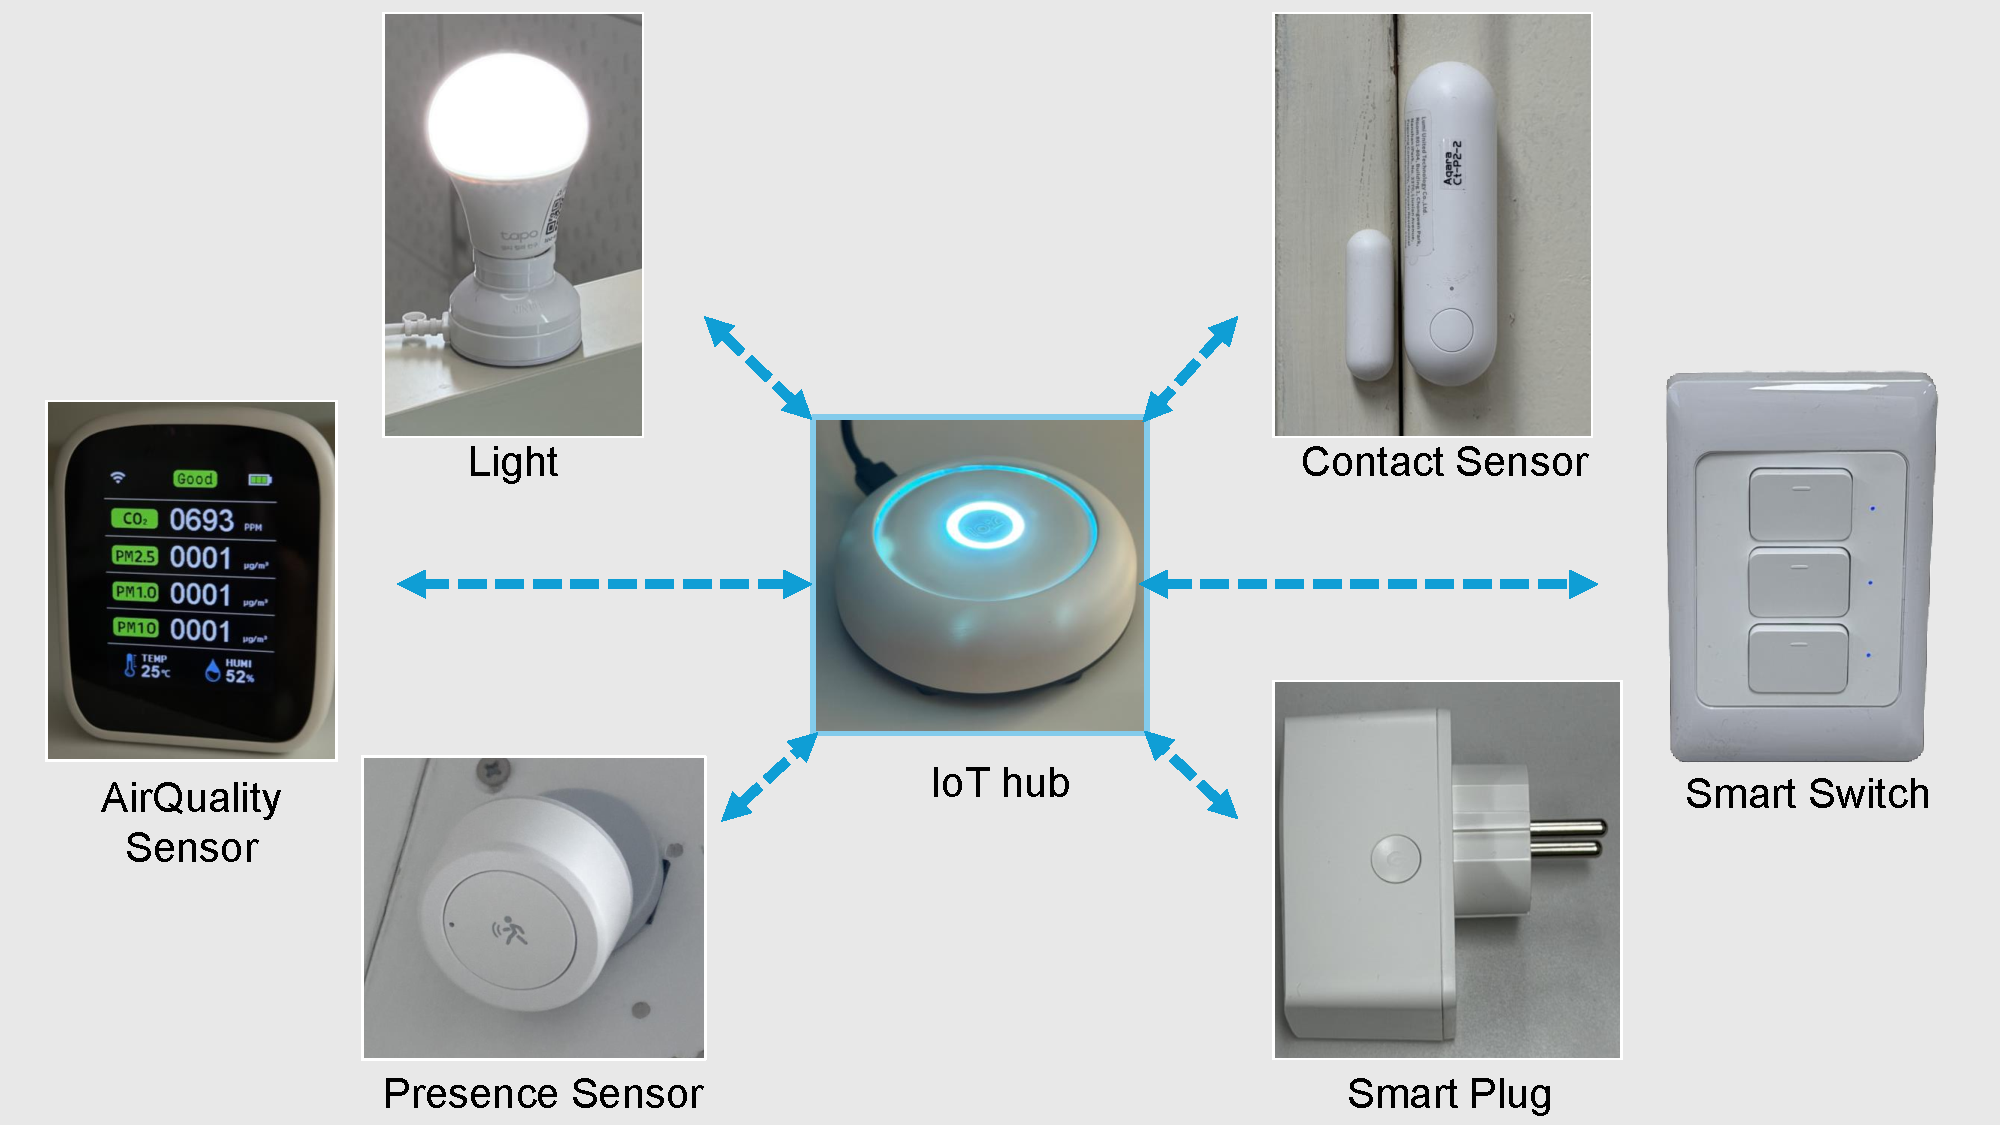
\includegraphics[width=.95\linewidth]{figs/Environment.pdf}
\caption{실물 테스트베드: 배포 시연에 사용된 센서·액추에이터를 갖춘 상용 엣지 허브.}
\label{fig:testbed}
\end{figure}

\textbf{Deployment.} Raspberry Pi 기반 엣지 허브와 실물 기기(presence·contact·공기질 센서; 플러그·조명·스피커; 그림~\ref{fig:testbed})를 갖춘 상용 홈 자동화 플랫폼(리뷰를 위해 이름 비공개)에서, 전체 파이프라인(IR 추출, 확인, lowering, 게이트)을 통해 여섯 개의 새 명령을 라이브로 작성하고 게이트 승인된 lowering을 등록했다. 이는 통계가 아니라 존재 증명이다.

표~\ref{tab:deploy}가 등록된 6개 자동화의 idiom, gate 결과, 관측 trace를 요약한다. 모든 관측 action 시퀀스가 플랫폼의 로깅 해상도에서 IR 예측 trace와 일치했으며, 하지 \emph{않아야} 할 것의 관측까지 포함한다(counted cycle이 정확히 3회 안내 후 정지; 교차한 임계가 높게 유지되는 동안 재안내 없음). 그림~\ref{fig:rq4}는 첫 행 ``회의실에 5분 이상 아무도 없으면 TV 플러그를 꺼줘''의 관측 trace다. 관측 대상은 TV 플러그 off action이 발화하는 시각이다: ungated lowering은 방이 빈 지 30초에 발화하고 — ungated 생성 4개 전부가 이 sustain 결함을 가졌다 — gate-repaired lowering은 IR이 예측한 5:00에 발화한다. authoring은 상류 게이트들도 행사했다: 초기 워딩 둘이 one-shot 조건 IR을 만들었는데 그 rendering이 확인 단계에서 오독을 드러냈고, 카탈로그 밖 타깃 하나는 추출 검증에서 fail-closed로 기각됐다.

\begin{table}[t]
\centering
\caption{실물 테스트베드의 라이브 작성 자동화: 게이트 결과와 예측-관측 거동.}
\label{tab:deploy}
\small
\setlength{\tabcolsep}{2.5pt}
\begin{tabular}{llll}
\toprule
Automation & Idiom & Gate & Observed \\
\midrule
presence absent 5min → TV plug off & sustain & repaired & off at 5:00 \\
speak every 30s, 3 times only & count & pass & 3 only, stops \\
door opens → light on & edge & pass & immediate \\
light off, on after 3min & delay & pass & on at 3:00 \\
CO\textsubscript{2} rises above 900 → announce & rising & pass & on crossing only \\
temp.\ rises above 28° → switch on & rising & pass & on crossing only \\
\bottomrule
\end{tabular}
\end{table}

\begin{figure}[t]
\centering

\includegraphics[width=.92\linewidth]{figs/deployment.pdf}
\caption{표~\ref{tab:deploy} 첫 자동화의 관측된 TV 플러그 off 시각: ungated lowering은 방이 빈 지 0:30에, gate-repaired lowering은 IR이 예측한 5:00에 발화한다.}
\label{fig:rq4}
\end{figure}

\section{Limitations}

가장 큰 한계는 NL→IR 의도 정확성이 열린 문제로 남는다는 것이다(Layer A). 사용자가 잘못 표시된 IR을 승인할 수 있고, 그 경우 verifier는 잘못된 spec에 충실히 검사한다. 이번에는 인간 확인 행동을 연구하지 않는다; rendering이 결정론적이고 충실한 평문 표면이라는 것까지만 확립한다. Ethics: 인간 참가자 데이터는 수집되지 않았다(``Not applicable: no human participants'').

그 외의 한계는: coverage 상한(counter-modulo guard의 else쪽; \S8.2); 경계 집중 동치는 입력 공간 전체 보장이 아님(다만 \S8.3의 dense 재심이 배포분에서 이 잔여를 측정한다); 유계 7일 horizon; 연속 산술(SMT는 future work); 값이 인자로 흘러가는 산술 — 값-특이 버그가 살아남을 수 있음(soundness가 아닌 coverage 한계; \S6.5); selector-free IR에서 같은 service의 두 read가 하나의 기기 키로 합쳐지는 것(precision은 이 논문 scope 밖); 단일 플랫폼 너머의 일반화.

\section{Conclusion}

reactive-temporal IoT 자동화는 LLM으로 생성하기 쉬워졌지만, 그것이 배포해도 되는 코드인지 결정하는 단계는 비어 있었다. OVLA는 LLM을 생성에 국한시키고 배포 게이트를 결정론적·LLM-free로 만든다: 사용자는 IR의 평문 rendering을 승인하고, 결정론적 검사기가 생성 코드를 그 승인된 IR에 대해 bounded trace-equivalence로 테스트하며, 어긋난 코드는 수리되거나 fail-closed로 기각된다. 382개 자동화에 걸쳐, 생성기가 만든 모든 어긋난 후보(최강 모델 기준 9.2\%)는 배포되는 대신 수리되거나 기각되었고, 게이트의 분류는 양방향 독립 재심 — 기각 전수 audit과 배포분 36,000회 무작위 dense 재실행 — 을 통과했다. 검증 루프에 LLM 없이, 엣지 기기 위에서다. OVLA는 자연어 의도 정확성을 해결하지 않지만, 사용자 승인을 통과하고도 살아남는 별개의 silent failure mode를 제거한다.

\balance
\bibliographystyle{ACM-Reference-Format}
\bibliography{refs}

\appendix

\section{Timeline IR Grammar}
\label{app:grammar}

Timeline IR은 각 step이 \texttt{op} 태그를 갖는 JSON 객체로 직렬화된다; 아래 문법은 abstract syntax를 EBNF로 제시한다. 터미널은 따옴표로 표시하고, \texttt{[\,x\,]}는 선택, \texttt{\{\,x\,\}}는 0회 이상 반복이다.

{\small
\begin{flushleft}
\texttt{ir \ \ \ \ \ \ ::= start\_at \{ step \}}\\
\texttt{step \ \ \ \ ::= wait | delay | read | call}\\
\texttt{\ \ \ \ \ \ \ \ \ \ \ | if | cycle | break}\\[3pt]
\texttt{start\_at ::= "start\_at" "(" ("now" | "cron" cron) ")"}\\
\texttt{wait \ \ \ \ ::= "wait" "(" expr ["," "edge:" edge]}\\
\texttt{\ \ \ \ \ \ \ \ \ \ \ \ \ ["," "for:" duration] ")"}\\
\texttt{edge \ \ \ \ ::= "none" | "rising" | "falling"}\\
\texttt{delay \ \ \ ::= "delay" "(" duration ")"}\\
\texttt{read \ \ \ \ ::= "read" "(" ident "," service "." attr ")"}\\
\texttt{call \ \ \ \ ::= "call" "(" service "." function}\\
\texttt{\ \ \ \ \ \ \ \ \ \ \ \ \ \{ "," name "=" (value | expr) \} ")"}\\
\texttt{if \ \ \ \ \ \ ::= "if" "(" expr ")" "\{" \{ step \} "\}"}\\
\texttt{\ \ \ \ \ \ \ \ \ \ \ \ \ ["else" "\{" \{ step \} "\}"]}\\
\texttt{cycle \ \ \ ::= "cycle" "(" "period:" duration}\\
\texttt{\ \ \ \ \ \ \ \ \ \ \ \ \ ["," "count:" ident]}\\
\texttt{\ \ \ \ \ \ \ \ \ \ \ \ \ ["," "until:" expr] ")"}\\
\texttt{\ \ \ \ \ \ \ \ \ \ \ \ \ "\{" step \{ step \} "\}"}\\
\texttt{break \ \ \ ::= "break"}\\[3pt]
\texttt{duration ::= int ("HOUR" | "MIN" | "SEC" | "MSEC")}\\[3pt]
\texttt{expr \ \ \ \ ::= expr ("or" | "and") expr | "not" expr}\\
\texttt{\ \ \ \ \ \ \ \ \ \ \ | arith [cmp arith]}\\
\texttt{cmp \ \ \ \ \ ::= "==" | "!=" | "<" | "<=" | ">" | ">="}\\
\texttt{arith \ \ \ ::= arith ("+" | "-" | "*" | "/") arith}\\
\texttt{\ \ \ \ \ \ \ \ \ \ \ | "abs" "(" expr ")"}\\
\texttt{\ \ \ \ \ \ \ \ \ \ \ | ("min" | "max") "(" expr "," expr ")"}\\
\texttt{\ \ \ \ \ \ \ \ \ \ \ | service "." attr | "\$" ident | literal}
\end{flushleft}
}

\noindent\texttt{service.attr}은 라이브 센서 읽기를, \texttt{\$}\texttt{ident}는 \texttt{read}나 \texttt{cycle.count}가 바인딩한 영속 변수를 나타낸다. \texttt{literal}은 숫자, 불리언, 기기 카탈로그가 선언한 enum 값을 포괄한다.

\noindent\emph{의미 규약.} \texttt{wait.edge="rising"}은 condition의 상승 교차마다 한 번 완료된다. \texttt{wait.for}는 condition이 그 duration 동안 연속으로 성립할 것을 요구하며 거짓으로 뒤집히면 리셋된다. \texttt{cycle.period}는 반복당 cadence이고, \texttt{until}이 없으면 cycle은 verifier의 유계 horizon 안에서 반복한다(\S6).

\noindent\emph{Context-sensitive 규칙 (문법 G, \S5).} step별 shape를 넘어 feasibility gate는 다음을 강제한다: (1) \texttt{timeline[0]}이 유일한 \texttt{start\_at}이다; (2) \texttt{start\_at}은 분기·루프 본문 안에 나타날 수 없다; (3) top-level \texttt{cycle}은 최대 하나이고 중첩 \texttt{cycle}은 없다; (4) \texttt{break}는 \texttt{cycle} 본문 안에서만; (5) \texttt{cycle.period}는 필수다. 카탈로그 적합성(모든 \texttt{Service.Attr}과 \texttt{call.target}이 연결 기기 카탈로그가 선언한 service·member·인자를 지칭하는지)도 같은 지점에서 검사되어 카탈로그 밖 타깃을 fail-closed로 기각한다.

\section{Dataset Category Breakdown}
\label{app:categories}

표~\ref{tab:categories}는 382개 명령 벤치마크의 24개 카테고리 분포다. 각 카테고리는 구조적으로 구별되는 reactive 패턴과 그 lowering idiom에 대응한다.

\begin{table}[h]
\centering
\caption{데이터셋 카테고리 (382 명령, 24 카테고리).}
\label{tab:categories}
\small
\setlength{\tabcolsep}{4pt}
\begin{tabular}{llr}
\toprule
ID & Pattern & n \\
\midrule
C01 & Single device action & 28 \\
C02 & Action with device selector & 33 \\
C03 & Single-condition \texttt{if} (incl.\ if-else) & 34 \\
C05 & AND-compound \texttt{if} & 30 \\
C06 & OR-compound / chained \texttt{if-elif-else} & 7 \\
C07 & Level-triggered wait (``when X, do Y'') & 32 \\
C08 & Rising-edge trigger (``whenever'') & 41 \\
C09 & Sequential delay & 18 \\
C10 & Trigger + delayed action & 9 \\
C11 & Snapshot, delay, and re-read comparison & 8 \\
C12 & Phase lifecycle (``when X, every N thereafter'') & 15 \\
C13 & Alternation / binary toggle & 7 \\
C14 & Progressive update with counter and stop & 7 \\
C15 & Cron-scheduled action & 21 \\
C16 & Cron + branch & 13 \\
C17 & Periodic polling + branch & 12 \\
C18 & Bounded duration (time-window cycle) & 10 \\
C19 & Hysteresis (double-threshold deadband) & 8 \\
C20 & Sustained condition (``for at least N'') & 17 \\
C21 & Group consensus (all/any quantifier) & 7 \\
C22 & Counted repetition (``repeat N times, stop'') & 10 \\
C23 & Sustained trigger + multi-step sequence & 5 \\
C24 & Sustained trigger + repeating alert & 5 \\
C25 & Periodic polling + if-else & 5 \\
\midrule
 & Total & 382 \\
\bottomrule
\end{tabular}
\end{table}

\end{document}
